% Chapter Template
\chapter{Event reconstruction in CMS} \label{Chapter2_5} 



This chapter outlines the main features of the CMS event
reconstruction. In Section~\ref{sec:reconstruction}, an explanation of
the reconstruction algorithm, called \emph{Particle flow} is
given. Thus they are discussed the reconstruction performances. The main focus of Section~\ref{sec:reconstruction} will be on lepton (electrons and muons) identification and
reconstruction in consideration of the multilepton final states which are
discussed in Chapter~\ref{Chapter5} and~\ref{Chapter6} and thus are
central to this dissertation.


\section{Event reconstruction}\label{sec:reconstruction}
With the term ``event reconstruction'' we mean the identification of
all final state particles which are produced in a proton-proton
collision. Particles are classified according to their distinct
signatures they leave in 
the CMS detector, as displayed in Figure~\ref{fig:cmsslice}.

\begin{figure}[h]
\centering
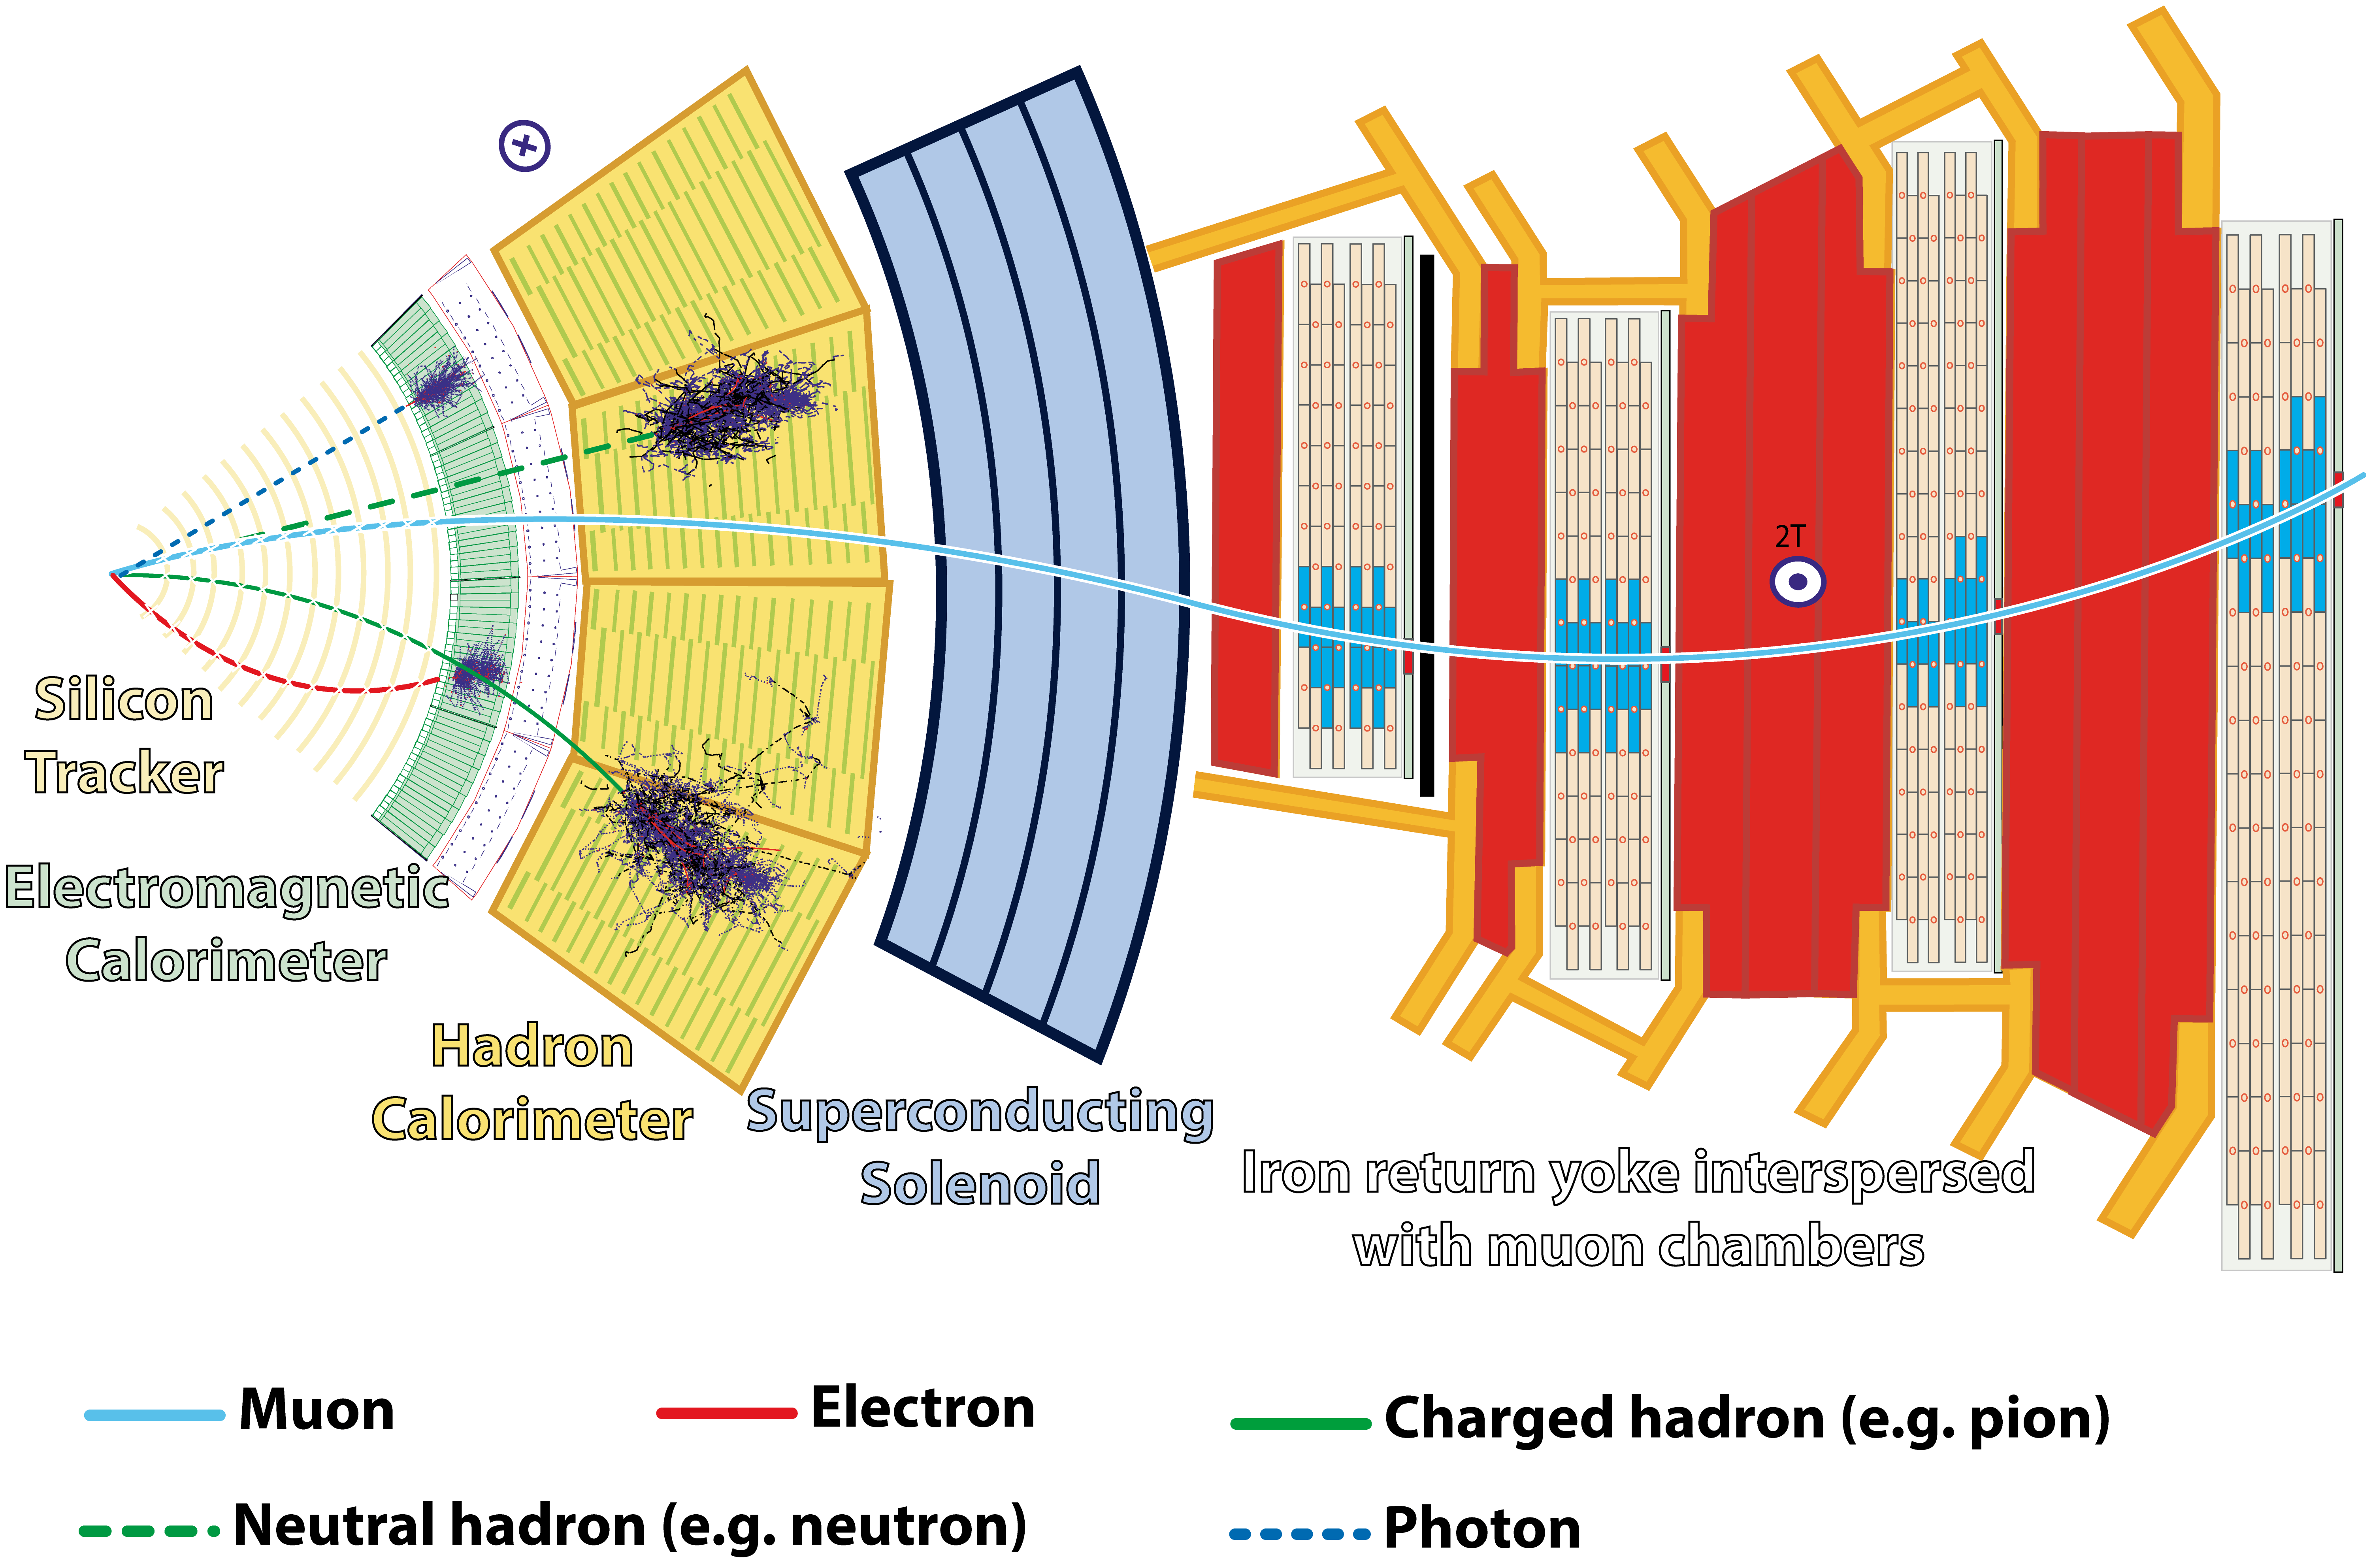
\includegraphics[width=0.88\textwidth]{Figures/c2/CMSslice.png}\\
\caption{Geometric view of a transverse slice of the CMS detector showing its sub-detectors and how particles interact with them~\cite{Barney:2120661}.}
\label{fig:cmsslice}
\end{figure} 
CMS detector is built with the idea of cylindrical detection layers
which are wrapped around the beam axis. After the collision, starting
from the point where the interaction occurs, particles enter in the
tracker. In the tracker, the charged-particle trajectories, \emph{tracks}
and their origins, \emph{vertices} are reconstructed using the information from
electronic signals, \emph{hits}, in the detection layers. Subsequently
electrons and photons are absorbed and stopped in the ECAL, while
charged and neutral hadrons, after eventually starting a hadronic
shower already in the ECAL, are fully absorbed in the HCAL. Finally muons and neutrinos cross
the full detector with little or zero interactions. The muons 
produce in the the muon-system signal hits and their trajectory is finally defined. This simple
event-view is graphically displayed in Figure~\ref{fig:cmsslice}.


This approach has led to the practice of reconstructing, in the first place, \emph{physics
objects} using the signals collected by a specific
detector.
An crucial improvement on the event description is obtained by
correlating (\emph{linking}) the basic \emph{elements} (\ie tracks and
clusters) from all the sub-systems. Thus each final-state
particle is classified and then the physics-object properties like
mass and momentum are reconstructed by combining the information from
the sub-systems. This
integrated approach is called \emph{particle flow} (PF)
\emph{reconstruction}~\cite{CMS:particleflow} and it is going to be
explained later in Section~\ref{sec:PF}.

\vspace{0.7cm}


This chapter details the approach and the relevant steps of the CMS
event reconstruction algorithms, paying particular attention to the
aspects pertinent to this thesis (i.e. light leptons). The track and vertex reconstruction 
is presented in Section~\ref{sec:trackvertex} and particle-flow
algorithm is described in Section~\ref{sec:PF}. Identification and
performances of muons and electrons are presented in
Sections~\ref{sec:trackmuon} and~\ref{sec:c2ele}.\\
Furthermore, some
effort is dedicated to the displaced lepton reconstruction in
Sections~\ref{sec:c2muondisplaced} and~\ref{sec:c2dispele} which is going to be central for the
analysis overview presented in Chapter~\ref{Chapter6}.\\

A topical distinction between the terms \emph{prompt}, \emph{nonprompt} and
\emph{displaced} leptons is needed before continuing with this
dissertation. With the definition \emph{prompt leptons}, we refer to
leptons that originates from primary
interaction vertex of the hard scattering collision and they come from
from interesting physics phenomena. \emph{Nonprompt leptons} are leptons from heavy-flavor decays, misidentified hadrons, muons from
light-mesons that decay in flight, or electrons from unidentified
conversions of  photons in jets. Both prompt and nonprompt leptons
(they will be called also fake leptons) are assumed to be originated
in proximity of  the beam
spot. Thus, the reconstructed variables giving an estimation of the
impact paramter have very small values. \emph{Displaced leptons} are
leptons that originate from a separate vertex with respect to
the primary interaction vertex. They are the results of the decay of 
particles which have lifetime ``long'' enough to travel from few mm up
to m far from the collision point.

\subsection{Track and vertex reconstruction}\label{sec:trackvertex}

Precise reconstruction of interaction vertices and charged
particle tracks is a crucial element for an accurate measurement of
charged particle momenta and properties. Moreover tracks, vertices and their
successive combination constitute an important input for pileup
mitigation (Section~\ref{lhc}) and for the
identification of displaced vertices where long-lived particles decay.
Finally tracks and vertices are fundamental inputs to the
particle-flow (PF) algorithm (Section~\ref{sec:PF}). \\

The tracking algorithms are devised to
increase the track-finding efficiency while keeping small the
contamination of fake tracks, \ie tracks constructed from uncorrelated hits or
including false hits.\\
 The tracks are reconstructed starting from the hits in the pixel and
strip tracker. The hit reconstruction follows two steps: the first,
indicated as local reconstruction, is a clustering of signals in the
tracker sensors. Thus 
the first estimate of the
position of the hit is determined based on the geometry of the single
pixel or strip while taking into consideration the Lorentz drift due
to the magnetic field (more detailed info about local reconstruction
can be found here:~\cite{CMS:particleflow}). The second step is a more
sophisticated reconstruction which uses the informations about the
irradiation status of the pixel and strip sensors. \\
The hit efficiency is measured to be above the 99.5\%\footnote{The hit
  efficiency depends on the
$d\mathcal{L}/dt$ and on the trigger rate, in particular in
the first layer of the pixel sub-detector where the occupancy is greater.} for both pixel
and tracker hits~\cite{CMS:particleflow}. According to the size of the
cluster and the angle of
incidence of the particle, the final resolution in the
hit position is measured to be in the range of 20 (10) and 50 $\mu$m
for the pixel (strip) tracker~\cite{CMS:particleflow}.\\
An additional input for the track reconstruction is the identification
of the LHC beam spot position, \ie the LHC luminous region's
3D profile, and the position of the collision
vertices. \\

The tracking algorithm used by CMS is called Combinatorial Track Finder (CTF)~\cite{Collaboration_2014_tracking}.
To lower the combinatorial complexity, it is applied an iterative
procedure in distinct successive iterations, each with moderate
efficiency and loosened selection requirements on the track quality with
respect to the step before. The Kalman
filter method~\cite{BILLOIR1990219} is used for the track-finding
algorithm. While taking into account the multiple Coulomb scattering on the
direction of the track, the Kalman filter makes use of track
seeds\footnote{``\emph{The seeds define the starting trajectory parameters and associated uncertainties of potential
tracks. In the quasi-uniform magnetic field of the tracker, charged particles follow helical paths
and therefore five parameters are needed to define a trajectory. Extraction of these five parameters
requires either three 3-D hits, or two 3-D hits and a constraint on the origin of the trajectory
based on the assumption that the particle originated near the beam
spot}''~\cite{Collaboration_2014_tracking}.} 
to extrapolate the track
trajectory to the successive detector module. Thus at each layer, new
additional consistent hits
are integrated into the trajectory and the track parameters are
calculated again. The procedure starts again and the new resulting
trajectory is extrapolated to the subsequent layer. At the end, tracks
which do not fulfill goodness-of-fit requirements are rejected. Tracks
which are ``easy'' to reconstruct, e.g. from particle with large \pt
(which means less evident curvature) and produced in proximity to the
interaction point, are reconstructed first. Therefore hits associated
to these tracks are taken out, making the subsequent iterations less
complex. To guarantee high efficiency, track-finding starts with
trajectory seeds which are built in the innermost region of the
tracker. 
The reconstruction efficiency for tracks with \pt $>$ 1\GeV  is measured to be larger
than 99\% for isolated muons for $|\eta| < $ 2.5 and between 80 and
99\% for electrons and pions~\cite{CMS:particleflow}. The track \pt
resolution depends on the \pt and $\eta$ of the tracks, and it is
lower than 1\% for muons with \pt $\in [1,10]$\GeV~\cite{CMS:particleflow}.\\

Vertices are reconstructed using the high-quality tracks which are
compatible with originating from the beam spot. They are then clustered
based on their coordinates along the \emph{z}-axis. An adaptive vertex
fitting~\cite{Waltenberger_2007} developed as an iterative re-weighted Kalman filter
is used to estimate the coordinates of the vertices. To each track a
weight between 0 and 1 is assigned according to the probability for that track to
belong to a specific vertex. Thus, vertex weights are appointed to each
vertex as the sum of the weights of all the
associated tracks, and the vertices with weights inferior with respect
to predefined
thresholds are rejected. The reconstruction efficiency depends on the
number of tracks associated to the vertex and it is estimated to
be close to 100\% for the cases with more than two tracks and around
98\% for vertices with two tracks~\cite{CMS:particleflow}. The
resolutions varies between 10 and 100
$\mu$m~\cite{CMS:particleflow}.\\
Among the multiple vertices that are reconstructed one is selected as
the most interesting collision to be analyzed. This so-called primary vertex (PV), is identified as the vertex with the largest
$p^2_T$ sum of all the physics-objects associated to it. The other vertices are assigned as pileup
vertices.

\subsection{The particle-flow algorithm}\label{sec:PF}

The PF algorithm~\cite{CMS:particleflow} is devised to cater a global event
description by linking and combining information from CMS
sub-detectors. 
\begin{figure}[h]
\centering
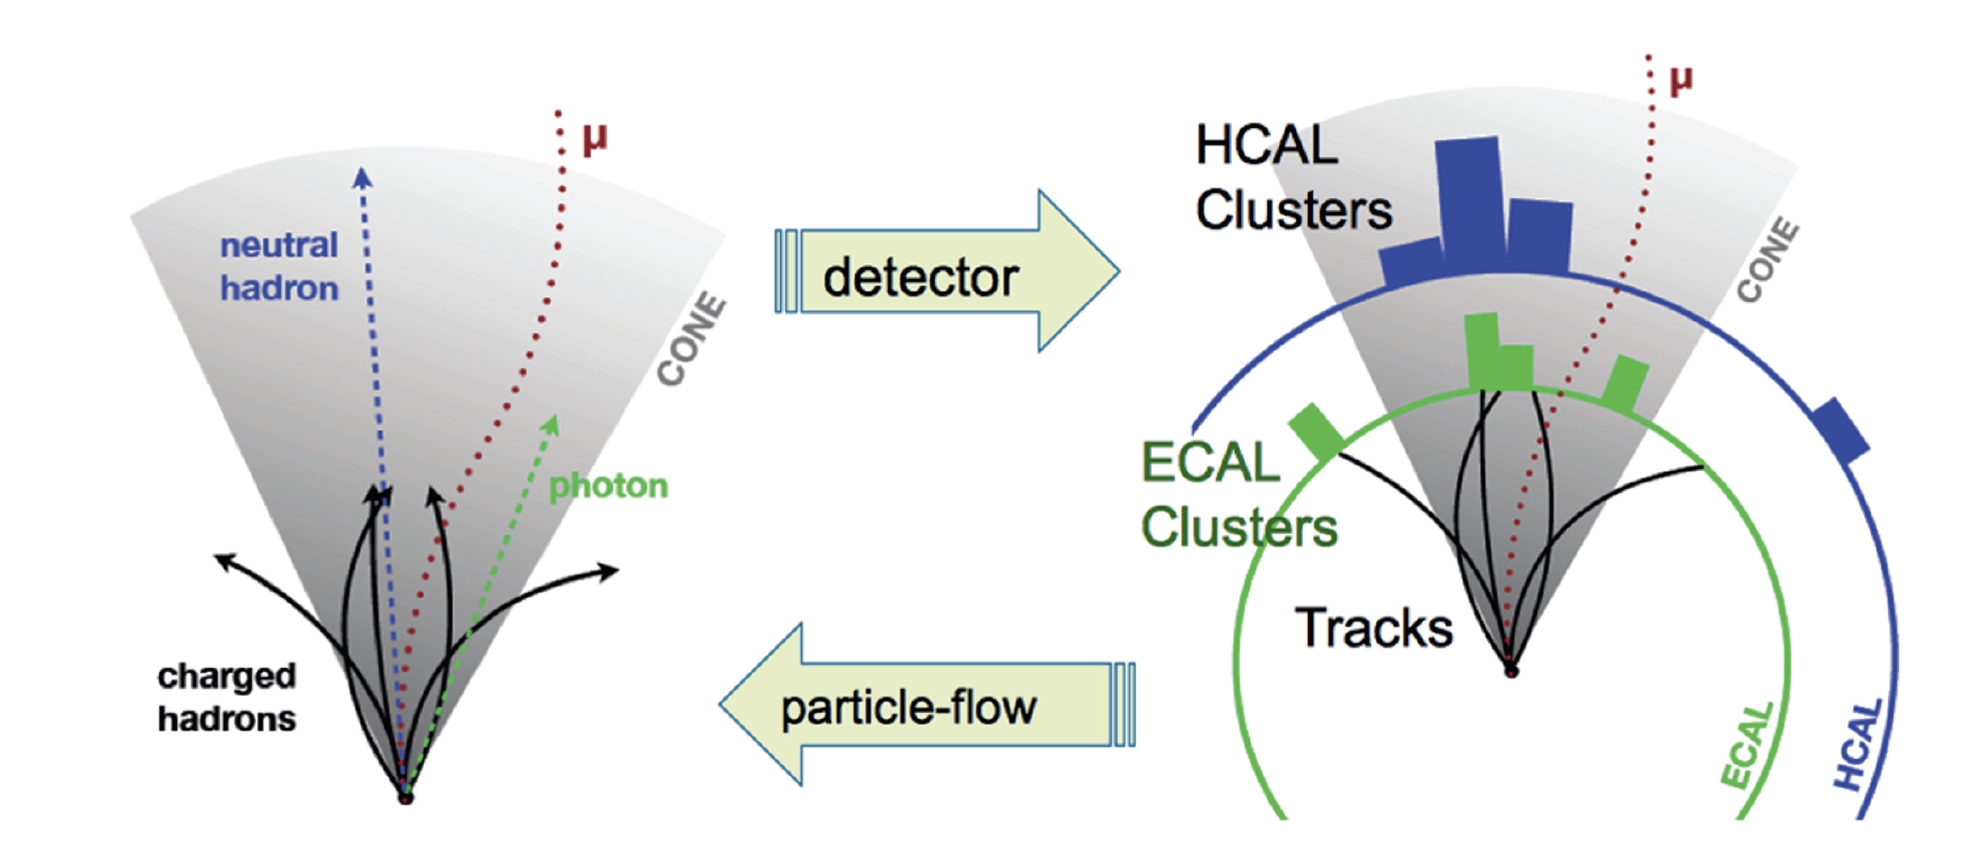
\includegraphics[width=0.78\textwidth]{Figures/c2/pfscheme}\\
\caption{The output of the PF is a list of candidates like
  electrons, muons, photons and hadrons. The PF algorithm links
  information from all the sub-system to give a global description of
  the collision event~\cite{Petrucciani:2650974}.}
\label{fig:pfscheme}
\end{figure} 

The input of the PF are the \emph{elements} such as tracks, vertices, tracks
reconstructed from the muon system and
calorimeter clusters. The output of the PF is a list of candidates
like electrons, muons, photons and charged and neutral hadrons (see
Figure~\ref{fig:pfscheme}). The identification of leptons, the
measurement of the \ptmiss and the categorization of the pileup tracks
are improved by the usage of the PF algorithm. When linking
information from tracker and calorimeters signals, noticeable gain is seen
in the momentum resolution of jets~\cite{CMS:particleflow}.

\subsubsection{Jet clustering and
  reconstruction}\label{sec:jetclustering}
As described in Section~\ref{sec:qcd}, quarks carrying a color
charge can neither exist nor be observed as individual asymptotic
states, hence they are always clustered with other colored objects around them
to make together colorless objects. The collection of these objects is name 
jet because the components all tend to fly in the same direction,
creating a "jet" of particles. This jet of hadrons originating from
quarks and gluons are then identified as PF candidates. 
To associate these jets of hadrons to the original particle a clustering algorithm is used.
Jets reconstruction is performed with a recombination algorithm which
is known as anti-$k_T$ algorithm (with distance parameter of the cone size
of $\Delta R = 0.4$). The detailed description of the anti-$k_T$ algorithm is not
discussed in this work but the information can be found in 
references~\cite{Cacciari_2008,Cacciari_2012}.

In order to reduce the number of jets rising from mis-reconstruction or
detector noise, identification requirements are applied depending on the single elements of the
jets \ie the number of particles and the amount of energy of the
jet which comes from different type of PF candidates~\cite{CMS-PAS-JME-16-003}.
The jet energy is set as the vectorial sum of the momenta of the
particles constituting the jet. In order to alleviate the effect of
pileup contribution in the jet reconstruction, charge hadrons
associated to pileup vertices do not enter in the jet clustering. This
scheme is known as ``charge hadron
subtraction''~\cite{CMS-PAS-JME-14-001} and removes a
considerable fraction of charged pileup particles.  
Subsequently it is applied a correction to account for the
contribution from neutral particles from pileup; the subtraction is
based on the average transverse momentum, \pt, per unit area in the
pileup jets~\cite{CACCIARI2008119, Cacciari_2008_area,
  Sirunyan:2020foa}.

Corrections on the jet energy are applied in order to correct for the
remaining pileup energy contributions and for any discrepancies
between jet properties in data and in simulated events. Those
correction are obtained from the ratio between the \pt of a
reconstructed jet and its corresponding generated jet and they are
measured as function of \pt and $\eta$ and applied to data and
simulation~\cite{Khachatryan_2017}. The jet \pt resolution is
derived both in data and MC and the resolution in the simulation is
fixed and smeared to match the one in the
data~\cite{Khachatryan_2017}.

\subsubsection{Tagging of jets originating from b
  quarks}\label{sec:tagging}
The identification of jets which originate from b quarks, called
\emph{b jets}, can be achieved using
specific properties and features of heavy
quarks inside the jet. This technique, usually called \emph{b tagging}, is
extremely important to discriminate between signal and background as
it will be explained in Chapters~\ref{Chapter5}
and~\ref{Chapter6}.

\begin{figure}[h]
\centering
    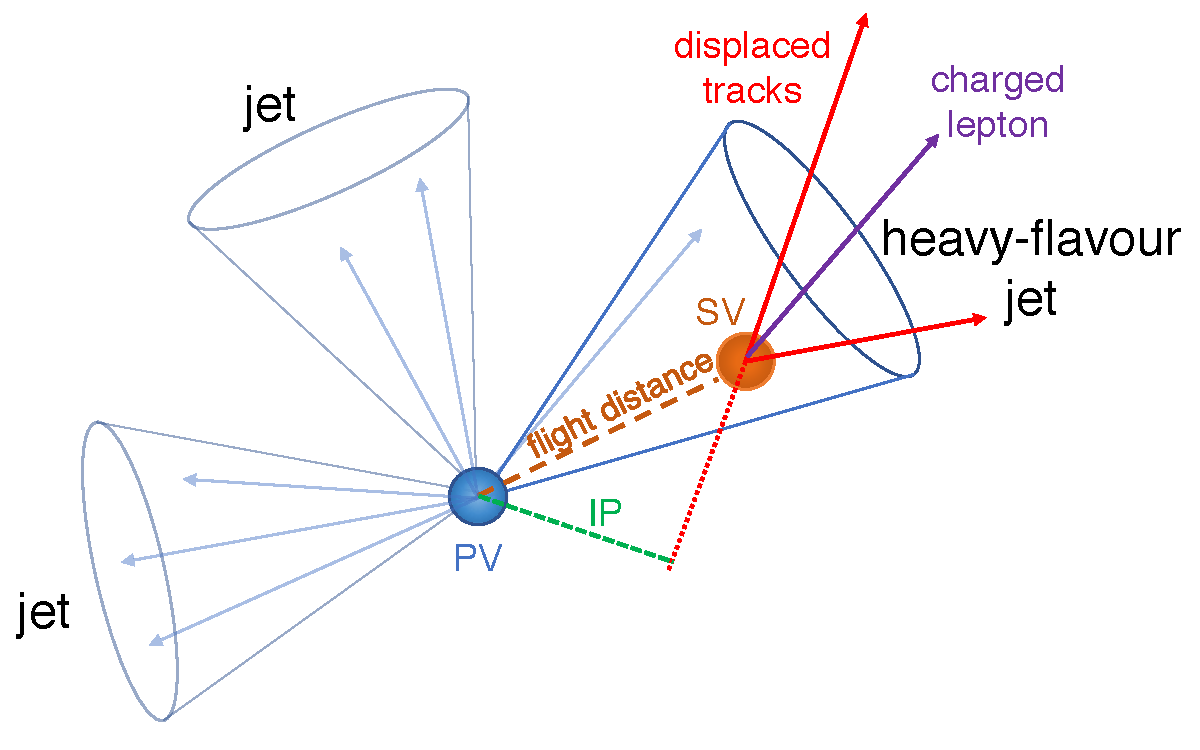
\includegraphics[clip,trim=0.3cm 0.5cm 0.3cm 0.3cm, width=0.50\textwidth]{Figures/c2/tagging}
  \caption{Schematic view of a b jet with a SV from the decay of a b hadron resulting in tracks which are displaced with respect to the PV, and hence with a large impact parameter (IP) value~\cite{Sirunyan_2018_tagging}.}
\label{fig:btagging}
\end{figure}

The b jets contain b hadron that have a lifetime of the order of 1.5
ps and a mass of about
5 $text{GeV}/c^{2}$. Thus the b hadrons can propagate from
the PV for a few mm up to one cm before decaying~\cite{Sirunyan_2018_btagging}. This results in
a secondary vertices (SVs) which contain displaced tracks, see
Figure~\ref{fig:btagging}. With respect to light jets (coming from
u, d, s quarks or gluons) b jets have larger mass and harder hadronization which
means that the decay products have larger momentum and larger number
of tracks related with the jet. These signatures are exploited by the
algorithms building variables to separate b jets from
light jets. The results of the b tagging are discriminator values, see Figure~\ref{fig:taggingperformance}; large discriminator values coincide with higher probability for
the jet to be a jet originating from b hadrons~\cite{CMS-DP-2017-013,
  csv}.\\
The b tagging performances are checked in terms of the b jet
efficiency (which expresses the fraction of all b jets truly coming from b hadron
that are identified as b jets) and of misidentification probability
(which expresses the fraction of light jets or jets from c hadrons
which are identified as b jets), see
Figure~\ref{fig:taggingperformance}. 

\begin{figure}[h]
\centering
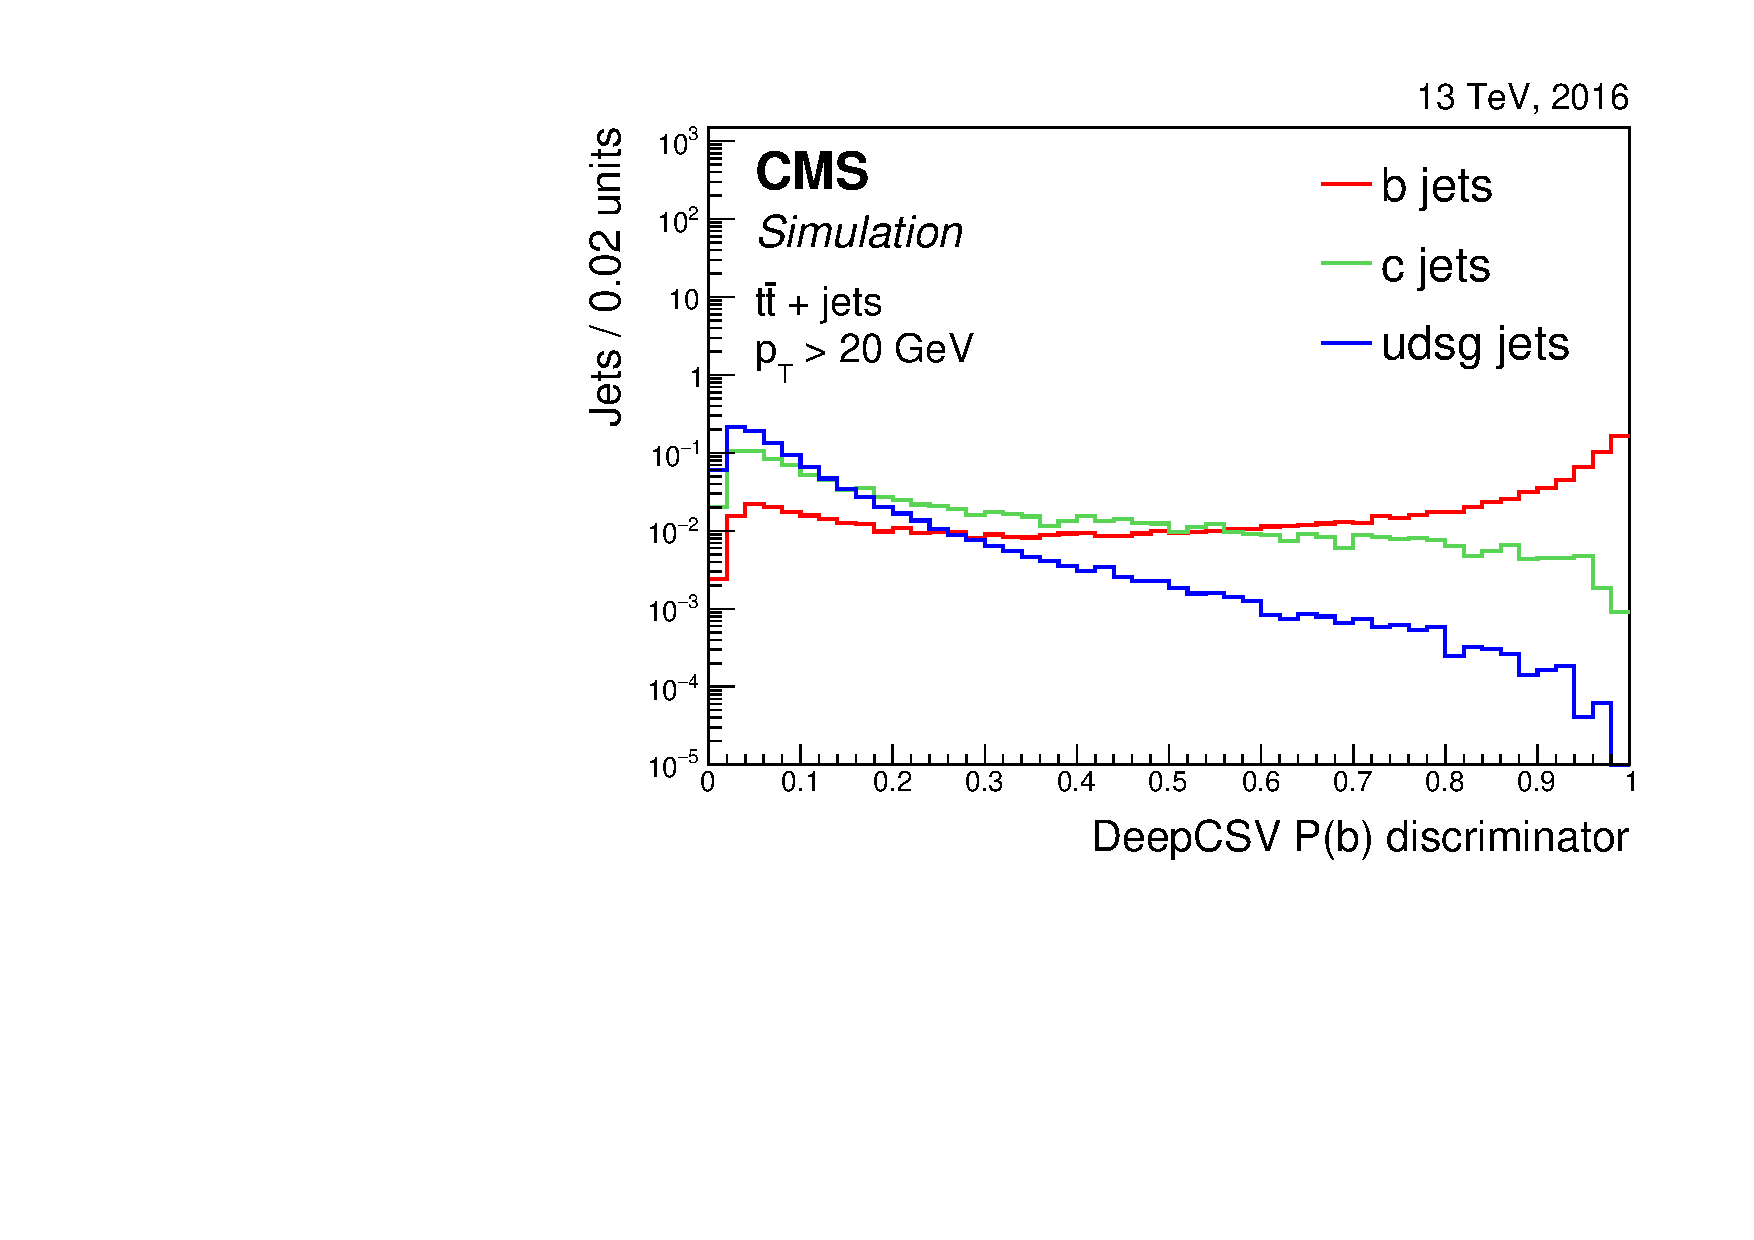
\includegraphics[width=.49\textwidth]{Figures/c2/CMS-BTV-16-002_Figure_013-a.pdf}
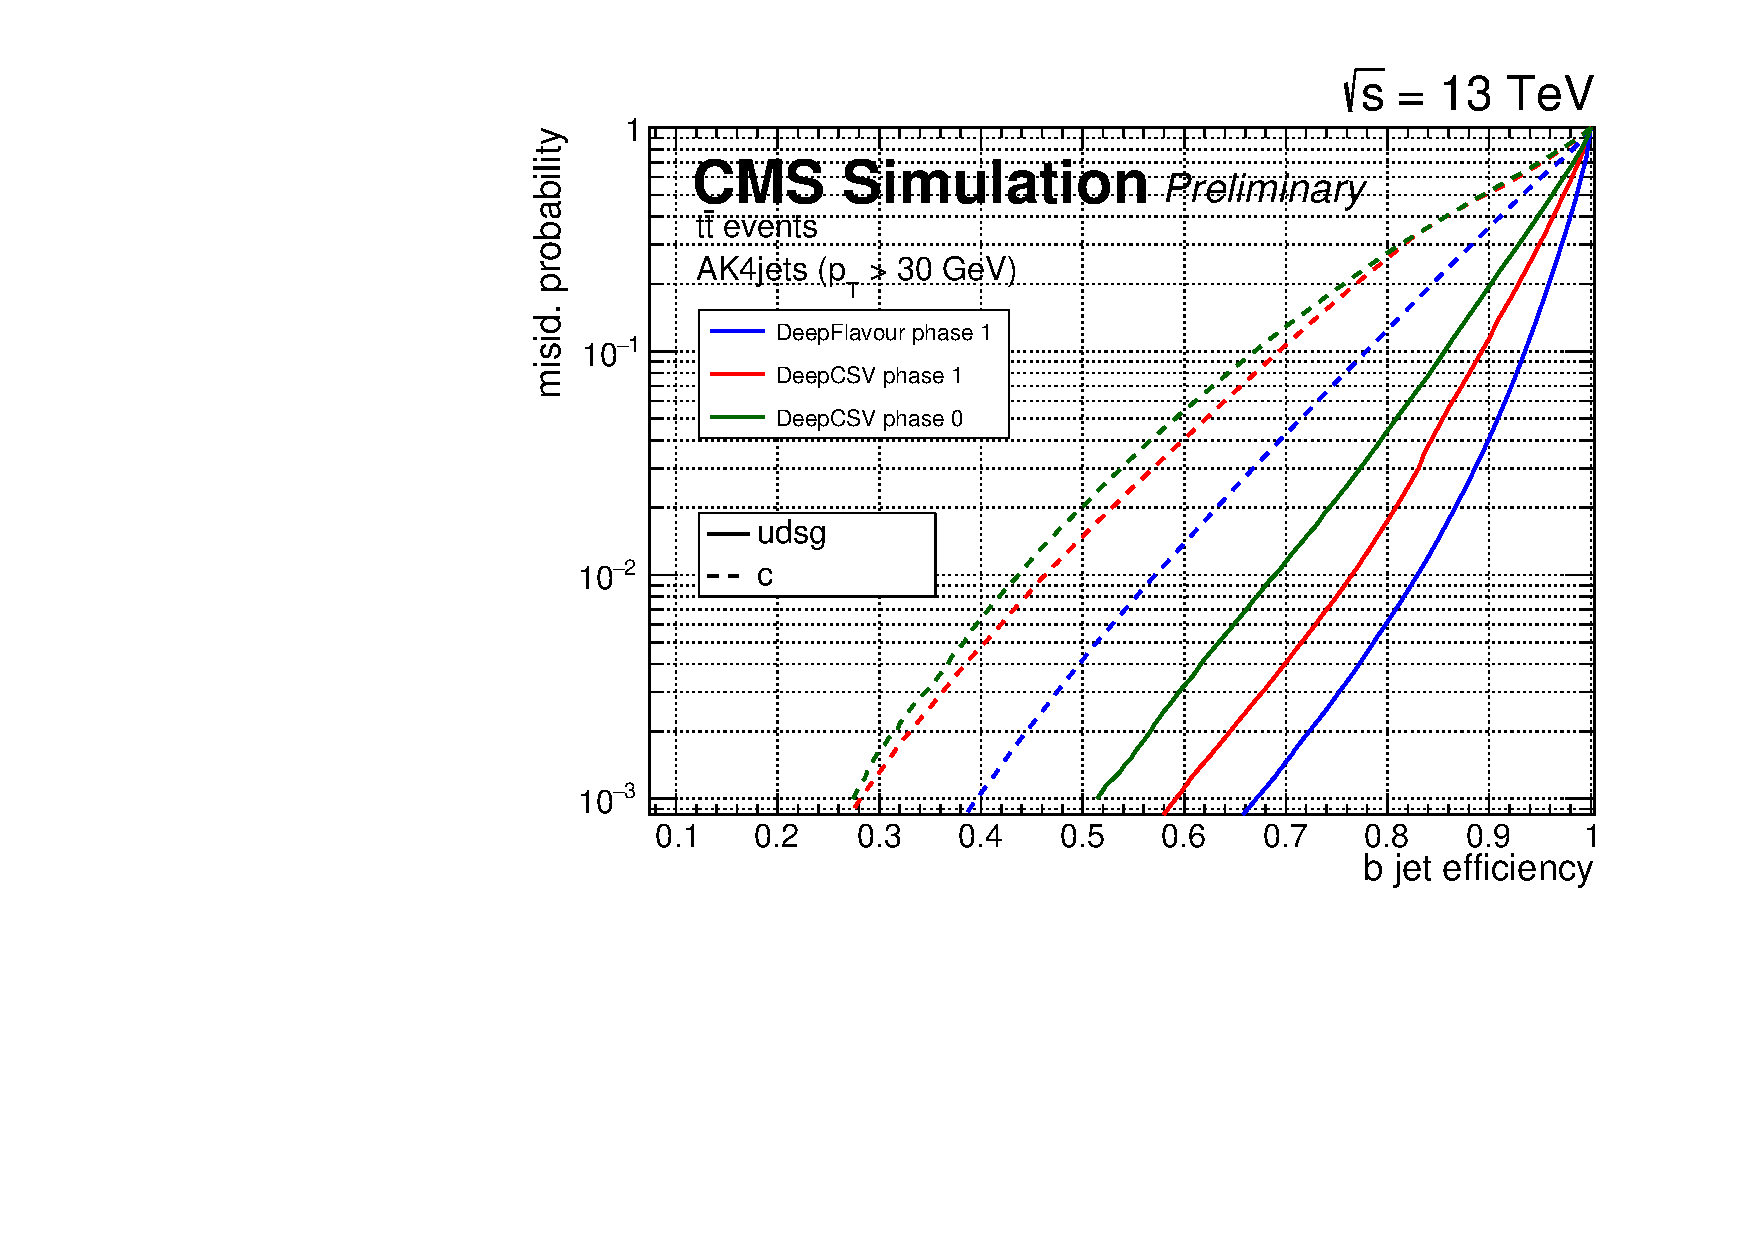
\includegraphics[width=.49\textwidth]{Figures/c2/PT30GeV.pdf}
\caption{On the left, ``performance of the DeepCSV and DeepFlavour b
  jet identification algorithms demonstrating the probability for
  non-b jets to be misidentified as b jet, as a function of the
  efficiency to correctly identify b jets. For comparison, the performance of DeepCSV
  with the 2016 detector (Phase 0) are also shown.''~\cite{csv}. On
  the right, ``Distribution of the DeepCSV P(b) discriminator values
  for jets of different flavors in \ttbar events. Jets without a
  selected track and without a secondary vertex are assigned a
  discriminator value of 0. The distributions are normalized to unit area''~\cite{csv}.}
\label{fig:taggingperformance}
\end{figure}

Here the two algorithms are known as DeepCSV~\cite{csv} and 
DeepJet~\cite{deep}. The first is the \emph{deep combined secondary vertex}, DeepCSV,
algorithm based on a fully-connected neural networks with a fixed set
of input variables for preselected tracks and preselected SVs and
kinematic features of the jets. The DeepJet~\cite{deep} is an improved
version of the DeepCSV. It is based on a deep neural network
architecture and it does not require any prior preselections and uses
a bigger number of SVs, tracks and neutral hadrons.
Looking at the right plot of Figure~\ref{fig:taggingperformance},
fixing the misidentification probability the DeepCSV has lower b jet
efficiency than DeepJet algorithm.\\
The efficiencies are calculated both in data and MC and the
corrections for the discrepancies observed between data and MC are
applied to simulated events as per-jet scale factors~\cite{csv}.


\subsection{Muon reconstruction}\label{sec:trackmuon}
This paragraph primarily describes the prompt muon reconstruction (~\ref{sec:c2muonselection}) and
identification (~\ref{sec:c2muonreco}). It will follow a description of the displaced
case and of the new improved algorithms which have been designed for these specific
scenarios (~\ref{sec:c2muondisplaced},~\cite{CMS-DP-2015-015}).

\subsubsection{Muon track reconstruction}\label{sec:c2muonreco}
Muon tracking~\cite{collaboration_2013,Sirunyan_2018_muon} makes use of information from
both inner tracker and muon systems. The
inner tracker gives a precise measurement of the muon momentum; the
muon system identifies muon objects over a wide acceptance with high efficiency. A high purity in muons is obtained
thanks to the upstream ECAL and HCAL which absorb other particles
(except neutrinos). \\
Three kinds of muon
candidates are defined according to the tracking algorithms that are used,~\cite{Sirunyan_2018_muon}:
\begin{itemize}
\setlength\itemsep{-0.2em}
\item \textbf{standalone muon}. The tracks are built from the
  information from all the muon sub-detectors, CSC, DT and RPC. It
  starts from seeds consisting of groups of DT or CSC segments, and
  the seeds are used for the pattern recognition in the muon system, to
gather all DT, CSC, and RPC hits along a muon trajectory using a
Kalman filter technique. The outcome of the fitting is called a
\emph{standalone-muon track}.
\item \textbf{tracker muon}. These tracks are formed
  ``inside-out''. They are extrapolated from the inner
  tracker to the muon system with loose matching to DT and CSC
  segments. Each inner track that has \pt$>0.5$\GeV and total
  momentum $>2.5$\GeV is extrapolated to the muon chambers and if at
  least one muon system segment matches that track than the muon track is defined as \emph{tracker
  muon track}. 
\item \textbf{global muon}. These tracks are built
  ``outside-in''. They are the results of the matching between
  standalone-muon tracks and tracker tracks. The matching is performed by
  comparing tracks parameters which are propagated onto a shared
  surface. Using data from both tracks, the final combined fit is performed with the Kalman filter technique.
\end{itemize}

About 99\% of the muons produced within $\eta < 2.4$ are reconstructed
either as a global muon track or as a tracker muon track (or
both). In case a global muon and a tracker muon share the same inner
track, they are then merged in one single candidate.
Global muons reconstruction is meant to be very efficient for muons
which penetrate
through more than one layer of the muon system. This implicitly
requires the muon track \pt to be more than 10\GeV since softer muons
easily fail this due to larger multiple scattering in the material of the return yoke; for the cases with
\pt$< 10$\GeV, the tracker reconstruction becomes then more efficient.
For muons which are not global muons and
they are matched with the innermost muon station only,
the probability for misidentification increases. The possibility for
hadron shower to reach the innermost muon station (punch-through)
becomes not negligible. In order to mitigate this effect additional
quality criteria on the muons are required at a later stage (described
in the following paragraph~\ref{sec:c2muonselection}).
By using the information from both the
inner tracker and the muon
system, the \pt resolution and measurement of global muons is improved
in particular for \pt $> 200$\GeV. For the case of standalone-muon
tracks, the muons have worse momentum resolution and a higher
contamination of cosmic muons than global or tracker muons.

Reconstructed muon tracks are given as input to the PF algorithm which
combines then all the information gathered from the different
sub-detectors. For muon case PF applies a list of selection criteria
to the candidates which have been reconstructed with standalone, track
and global muon algorithms. 

\subsubsection{Muon identification}\label{sec:c2muonselection}

Disparate sources of muons aside from the
prompt ones produced in the hard scattering collision can be spotted.
Muons can be
originated from either decay of heavy-flavor
hadrons or or cosmic-ray muons going through CMS detector, they can also appear from out-of-time pileup, beam
backgrounds and chamber noise which can compromise the reconstruction.
Implementing a selection based on quality and 
kinematic parameters is desirable in order to discriminate between different sources and to identify the
prompt muons from the hard scattering.\\
According to the desired compromise between efficiency and purity, it
is defined a set of different variables and selections definitions~\cite{Sirunyan_2018_muon}.\\
This level of details, here described, is going to be recalled and
used in Chapters~\ref{Chapter5} and in particular~\ref{Chapter6} where a customized and mindful selection is needed
for the displaced muon case (specifically Section~\ref{sec:llmuon}).

Some variables are related to the muon reconstruction itself. We can
list the \emph{track fit $\chi^2$}, the number of hits per track (it refers
to inner tracker hits, \emph{fraction of valid tracker hits}) and for global muons, the
level of \emph{position matching} between the tracker tracks and the standalone muon
tracks. Additionally the \emph{muon segment
compatibility} is an important parameter which returns values between 0
and 1 with 1 being the highest degree of compatibility. A \emph{kick
  finder} algorithm is deployed to evaluate a posteriori for each muon
track the
probability of being a single track or the combination of two
separated tracks.  \\
Other variables benefit from inputs from outside the muon track
reconstruction itself such as the track-PV compatibility.

Exploiting these variables, three main identification types of muons
are used in CMS physics analyses:
\begin{itemize}
\setlength\itemsep{-0.2em}
\item \emph{Loose muon identification, (Loose ID)}. A loose muon is either a
  tracker muon or a global muon. Loose ID tries to identify muons
  coming from the PV and from light and heavy flavor decay keeping
  very high selection efficiency and rather low misidentification rate
  of charged hadrons as muons. 
\item \emph{Medium muon identification, (Medium
    ID)}~\cite{PetruccianiBotta}. This selection aims to achieve, with
  respect to Loose ID, more rejection	
of muons from hadron decays in-flight while preserving
high selection efficiency. Medium muons are loose muons with tracker
tracks which have at least 80\% of valid hits in the inner tracker. 
If the muon is only a tracker muon (not a global muon), the muon
segment compatibility has to be larger than
0.451. If the muon is both a tracker muon and a global muon, ``the
muon segment compatibility need only be greater than 0.303, but then the global fit
is required to have goodness-of-fit per degree of freedom ($\chi^2$/dof) less than 3, the
position match between the tracker muon and standalone-muon must have $\chi^2$ < 12,
and the maximum $\chi^2$ computed by the kink-finding algorithm must be less than 20.
The constraints on the segment compatibility were tuned after application of the
other constraints to target an overall efficiency of 99.5\% for muons from simulated
\PW and \PZ events.''~\cite{Sirunyan_2018_muon}.
\item \emph{Tight muon identification, (Tight ID)}. A tight muon must
  be reconstructed both as global muon and tracker muon. With respect
  to the Medium ID, the Tight ID requirements are more stringent on
  the number of muon stations which have to match with the inner
  tracker track and on the compatibility between track and PV. 
\end{itemize}
There are other two identification types of muons, \emph{soft muon ID}
and \emph{high momentum muon ID} which are not used in the context of
this thesis and therefore are not detailed in this section. 


\paragraph{Reconstruction and identification
  efficiencies.}\label{sec:c2effmuon}

The efficiencies of the muon reconstruction and identification are
estimated in data and simulation events with a \emph{tag-and-probe}
method. The events are selected with two muons whose invariant mass,
$M_{\mu \mu}$, is compatible with the \PZ mass. 
\begin{figure}[h!]
\centering
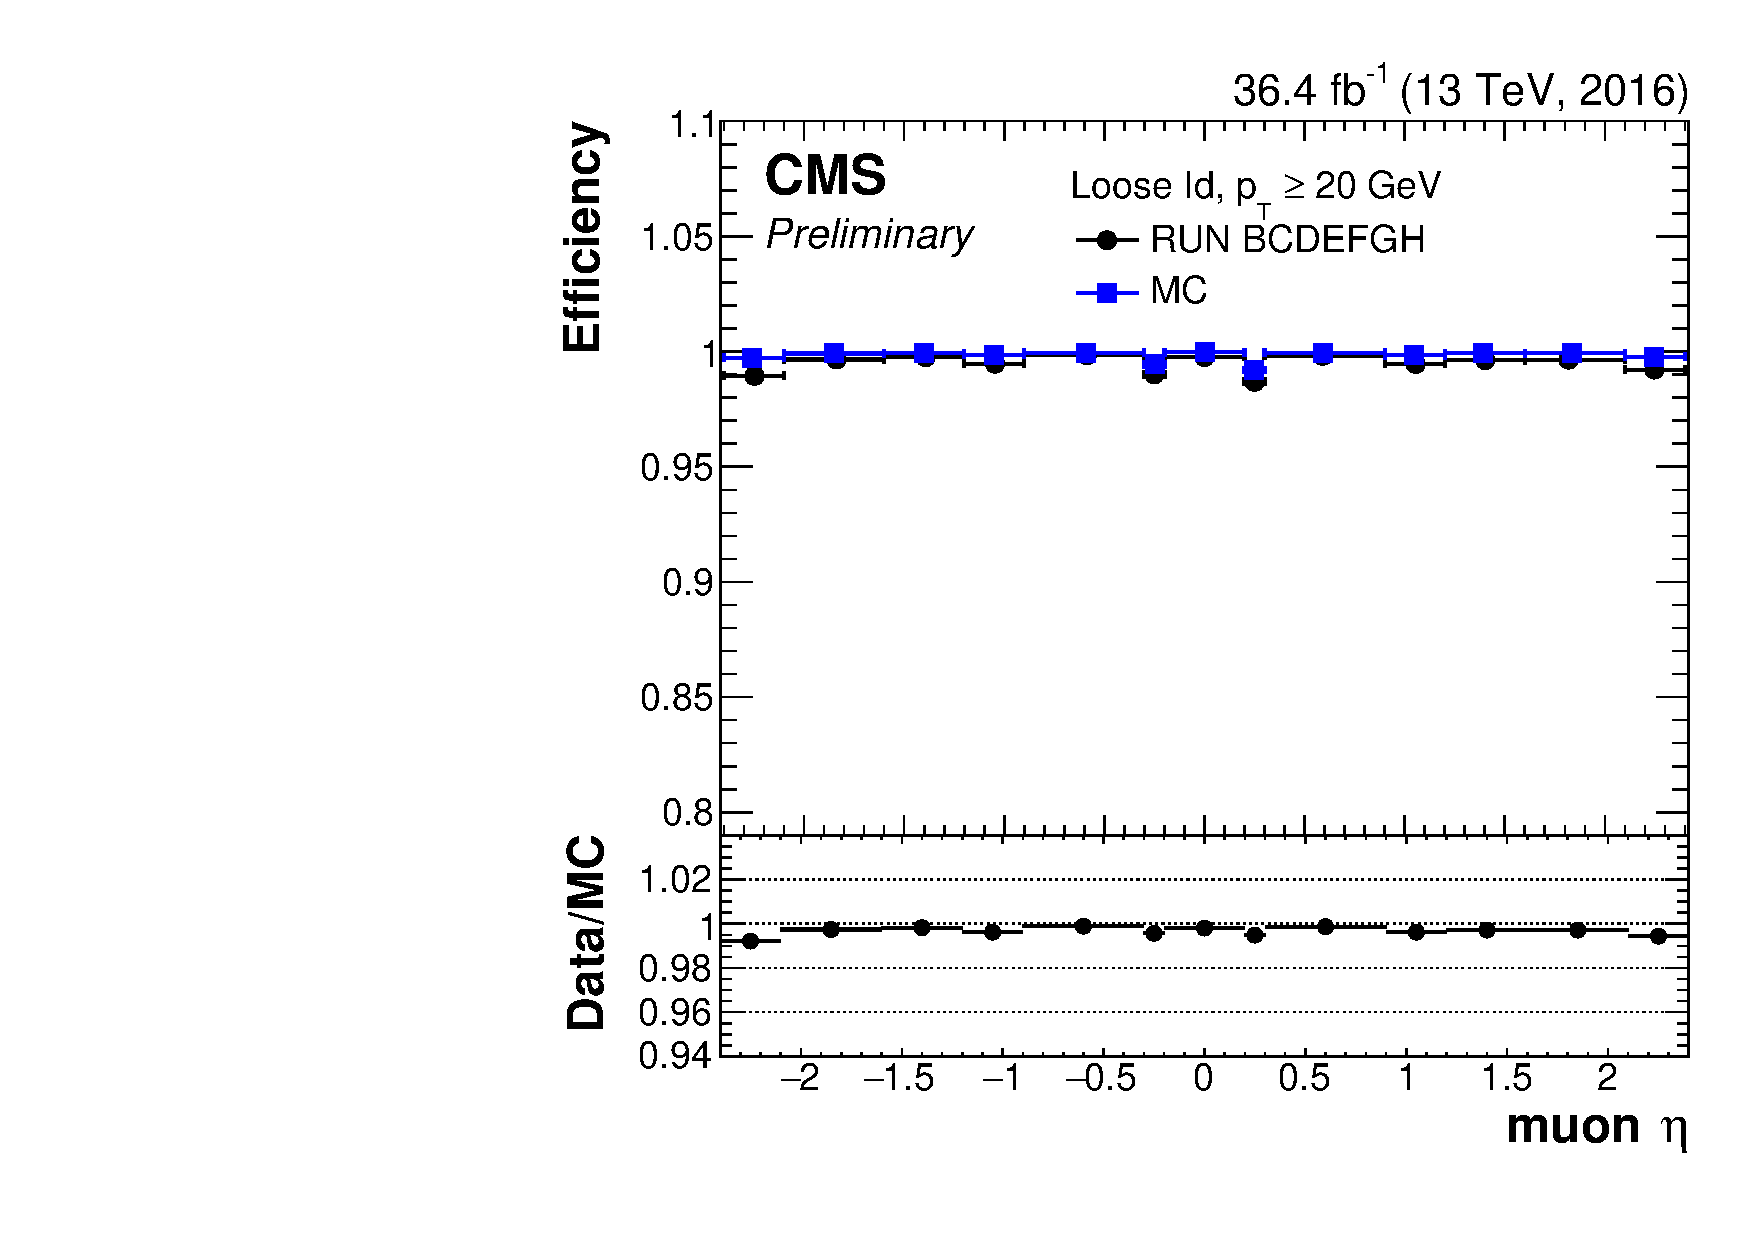
\includegraphics[width=.48\textwidth]{Figures/c2/TnP_MC_NUM_LooseID_DEN_genTracks_PAR_eta_.pdf}
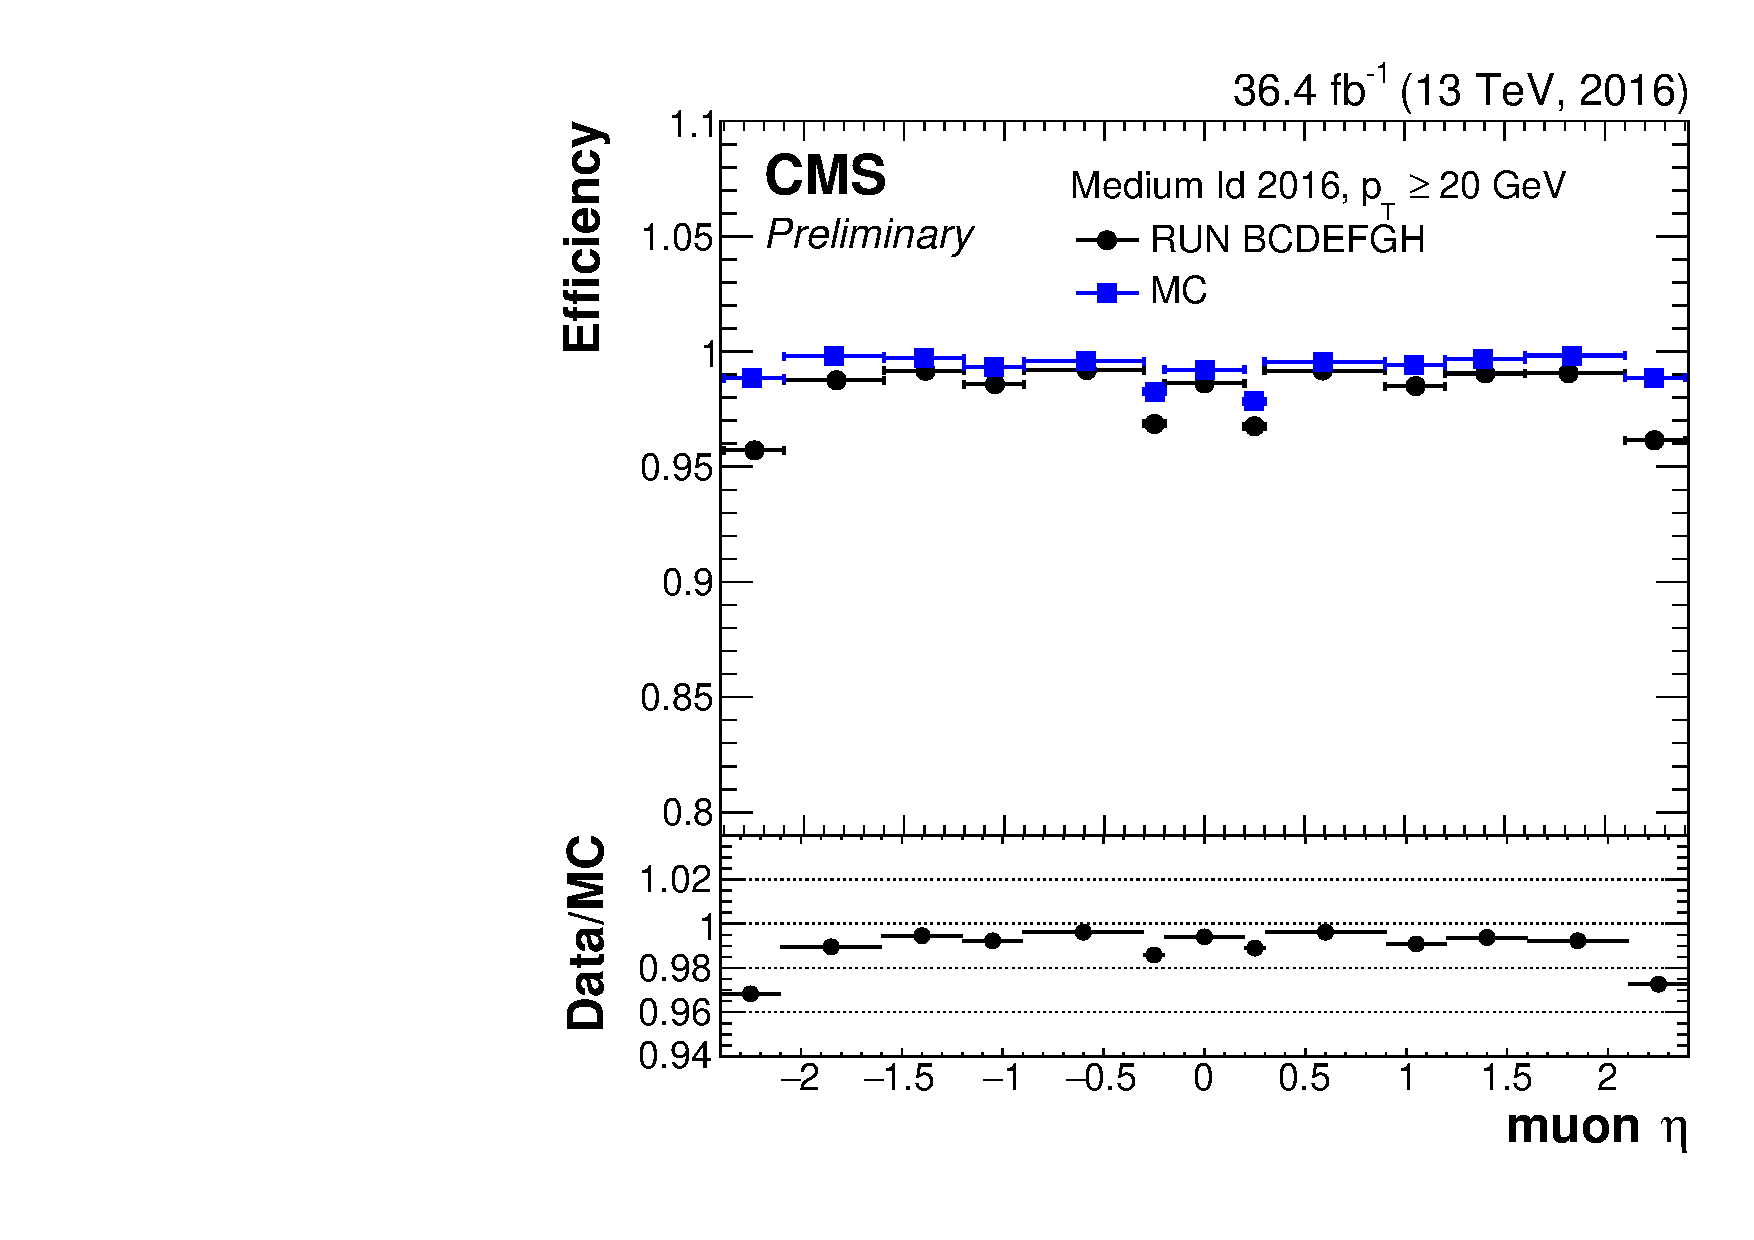
\includegraphics[width=.48\textwidth]{Figures/c2/TnP_MC_NUM_MediumID2016_DEN_genTracks_PAR_eta_.pdf}
\caption{Tag-and-probe efficiency for muon identification in 2016 data
  (circle) and simulation (squared). On the left, Loose ID efficiencies as function of $\eta$. 
On the right, Medium ID efficiencies as function of $\eta$. The
  denominator contains tracker muons. Error bars in the plots include only statistical uncertainty~\cite{CMS-DP-2017-007}}
\label{fig:2016eff}
\end{figure}
One of the two muons,
the \emph{tag}, is selected with tight requirements. The value of the
efficiency for a specific selection (reconstruction or identification
variables) is given by the fraction of the other muons, the
\emph{probes}, which pass that specific selection.The differences in
efficiencies between data and simulation samples are accounted and
then corrected with per-muon scale factors applied to the simulated
events~\cite{Sirunyan_2018_muon}. The performances of muon
reconstruction and identification in CMS using the data collected in
2016 are shown in Figure~\ref{fig:2016eff} (details and 2017-2018
results in the reference
here:~\cite{CMS-DP-2017-007,CMS-DP-2018-042}).

\paragraph{Muon isolation}\label{sec:muoniso}
To discriminate between prompt muons and muons coming from either the decays
of heavy-flavor hadrons or the decay in flight of charged $\pi^{\pm}$s and kaons, the isolation variable appears to be one of
the most critical variable to use. The PF isolation of a reconstructed
leptons is defined relative to its \pt as the scalar
sum of the energy of all the PF candidates emitted around the
direction of the muon in the cones, $\Delta R = \sqrt{(\Delta
  \phi)^2+(\Delta \eta)^2}$, surrounding the object. Detailed
information on isolation definition and isolation corrections are
given in Section~\ref{sec:c2variables}.

 \begin{figure}[h!]
\centering
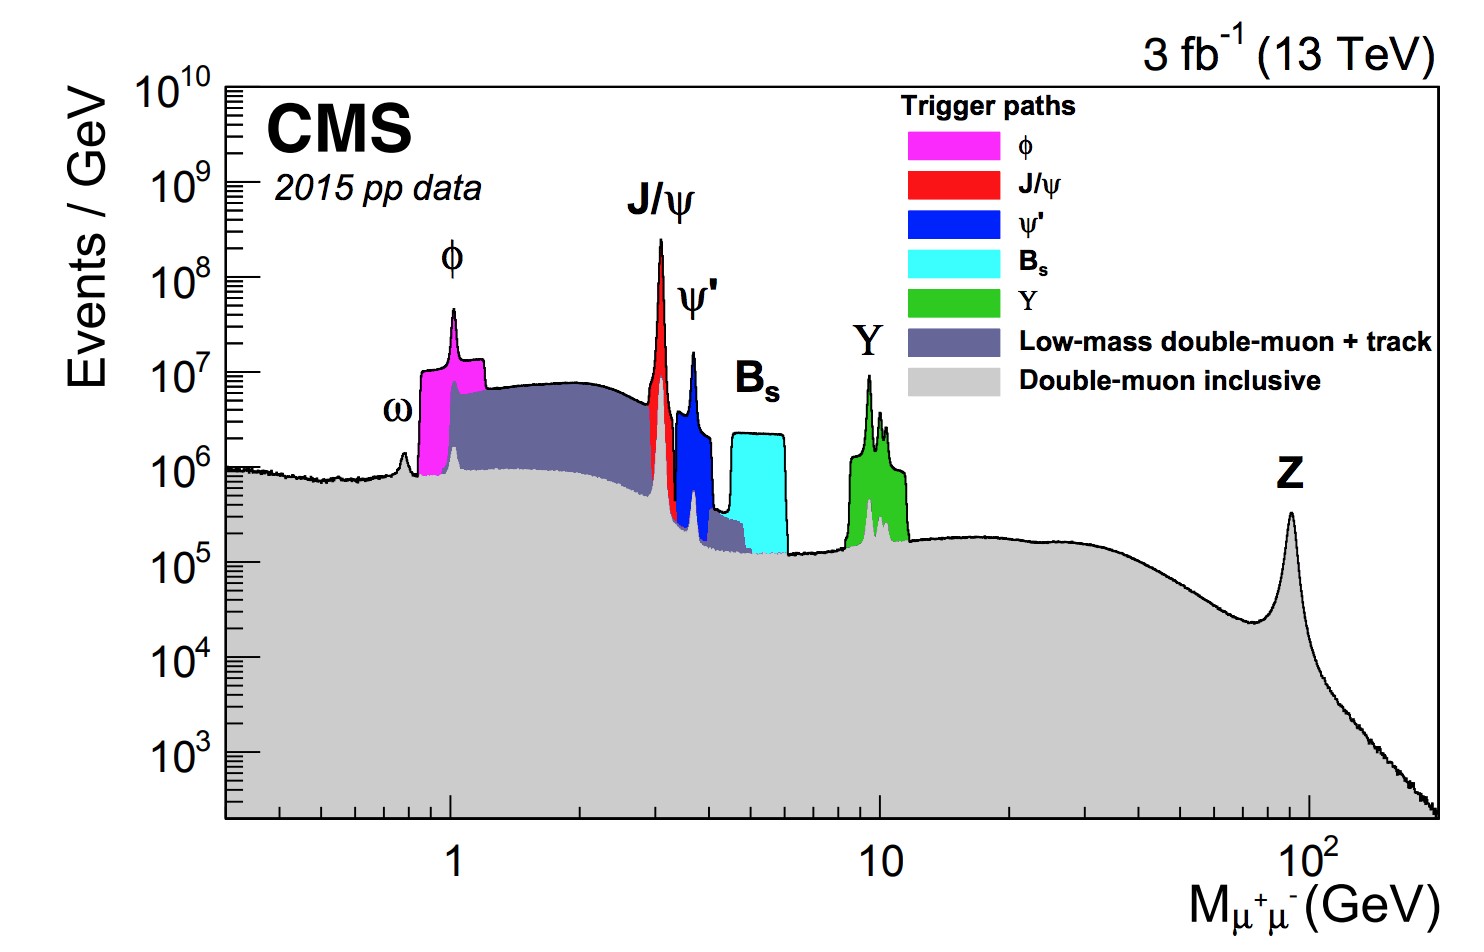
\includegraphics[clip,trim=1.2cm 0.1cm 0.5cm 0.3cm, width=.60\textwidth]{Figures/c2/dimuon}
\caption{``The dimuon invariant mass distribution reconstructed by the CMS HLT. Data were
collected in 2015 with the inclusive double-muon trigger algorithm (gray), as well as triggers
dedicated to selecting resonances at low masses.''~\cite{Sirunyan_2018_muon}.}
\label{fig:dimuon}
\end{figure}

Figure~\ref{fig:dimuon}, from reference~\cite{Sirunyan_2018_muon}, shows $M_{\mu \mu}$, the invariant mass distribution of dimuon pairs selected by
the inclusive trigger on isolated (for isolation definition refer
to~\ref{sec:c2variables}) double-muons. Specific triggers for low
invariant mass resonances are also included.\\
The distribution in Figure~\ref{fig:dimuon} clearly states
the CMS capabilities in identifying and trigger on
muons, reconstruct the muon properties to unambiguously
identify particles that decay into muons over a broad mass range.



\subsubsection{Displaced muon
  reconstruction and identification}\label{sec:c2muondisplaced}
The search for Heavy Neutral leptons presented in
Chapter~\ref{Chapter6} includes the long-lived heavy
 neutrino scenario with
displaced leptons, muons and electrons, in the final
state. Although CMS detector was initially designed and optimized for prompt
object reconstruction and identification, it appears to give
promising performances even for displaced lepton
reconstruction. Several studies and improvements on displaced physics object
reconstruction have been recently
delivered, helping in the challenging effort of including long-lived
exotic searches in the CMS results (~\cite{cmscollaboration2021search, Sirunyan_2019ll,
  Sirunyan_2019ll2, Sirunyan_2020ll, Sirunyan_2021ll,CMS:2021tkn}).\\

The analysis presented in Chapter~\ref{Chapter6} makes use of the
standard reconstruction which
 is explained in
Section~\ref{sec:c2muonreco}.

\begin{wrapfigure}{l}{0.5\textwidth}
\centering
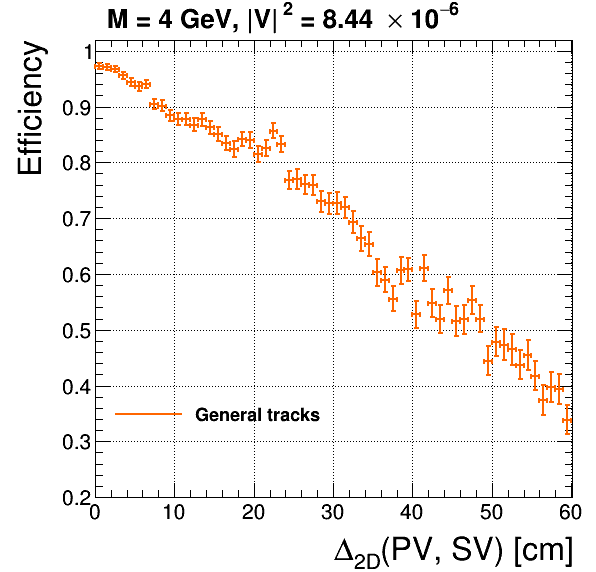
\includegraphics[width=.40\textwidth]{Figures/c6/object/tracking_M-4_V-0p00290516780927_rho.png}
  \caption{Efficiency of reconstructed inner tracker tracks with
    respect to generated muons. A HNL scenario with
    $(\mhnl,\mixparm)=(4\GeV,8.44\times10^{-6})$ is used as
    benchmark. \dani}
  \label{fig:c2tracking}
\end{wrapfigure}
In the following we present the studies of displaced muon
reconstruction and identification in the specific context of Heavy
neutral lepton search (refer to
Chapters~\ref{Chapter3},~\ref{Chapter4},~\ref{Chapter5},~\ref{Chapter6}).\\
These studies are performed with simulated samples containing
 low \pt displaced muons. 
The signal samples are characterized by HNLs with an
average life time of 57 mm ($c\tau$), which corresponds to an average
displacement of 633 cm ($\beta \gamma c \tau$).

Figure~\ref{fig:c2tracking} shows the efficiency of
reconstructing a muon track in the inner tracker. The efficiency is
calculated as pure reconstruction efficiency with respect to the
generated tracks. The variable that is used to display the reconstruction
performance is the 2-dimentional (2D) distance between the PV and the secondary vertex (SV)
and is a proxy to estimate the flight distance of the
displaced muon (details in Section~\ref{sec:c2variables}). The efficiency worsens for muons created towards the external layers of the inner
tracker.
\begin{figure}[h!]
\centering
  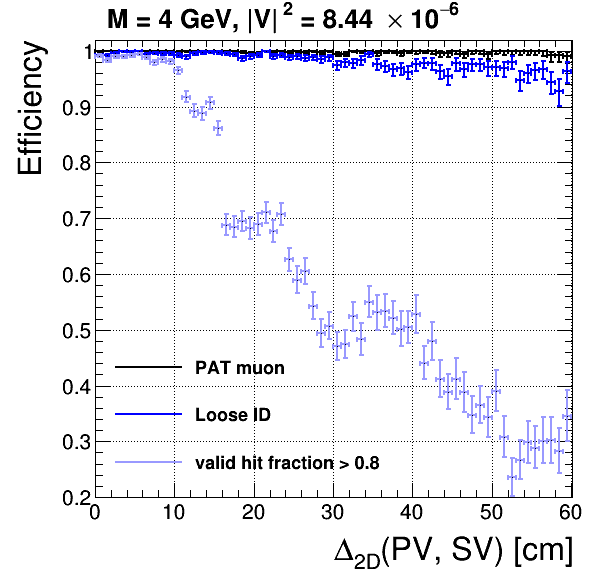
\includegraphics[width=0.4\textwidth]{Figures/c6/object/loose_validFraction_M-4_V-0p00290516780927_rho.png}
  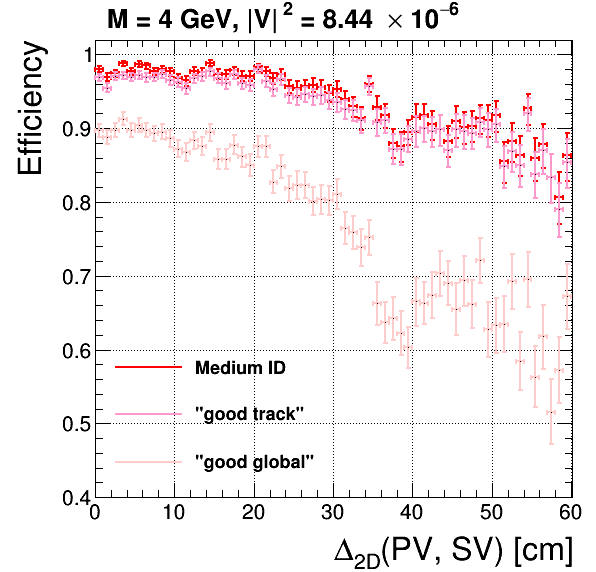
\includegraphics[width=0.4\textwidth]{Figures/c6/object/goodTrack_goodGlobal_M-4_V-0p00290516780927_rho.png}
  \caption{On the left, the sequential
efficiencies of the plain PF Muon requirement, Loose ID, and
valid tracker hit fraction requirement is shown. On the right, the efficiency of the tracker-muon only and
    global-muon only requirements is compared with their logical OR
    efficiency (using already the customized Medium ID). A HNL scenario with
    $(\mhnl,\mixparm)=(4\GeV,8.44\times10^{-6})$ is used as
    benchmark. \dani}
  \label{fig:c2tracking2}
\end{figure}

Figure.~\ref{fig:c2tracking2} shows, on the left, the sequential
efficiencies of the plain PF Muon requirement,
Loose ID, and
valid tracker hit fraction requirement (refer to
Section~\ref{sec:c2muonselection}), with respect to the reconstructed inner-tracker tracks. It is clear that the efficiency of
this last selection 
falls rapidly as the PV-SV
distance increases. 
The valid-hit fraction request is thus removed from the set of
requirements of the Medium ID (refer to
Section~\ref{sec:c2muonselection}). 
\begin{wrapfigure}{r}{0.5\textwidth}
\centering
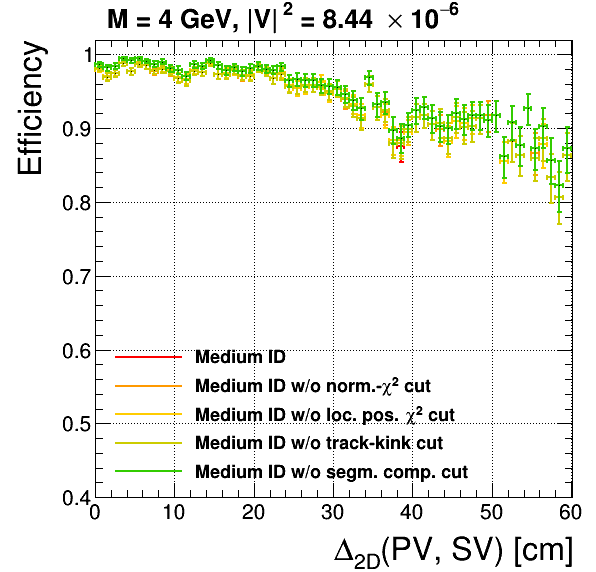
\includegraphics[width=.4\textwidth]{Figures/c6/object/globalTrack_cuts_M-4_V-0p00290516780927_rho.png}
  \caption{Efficiency of different Medium-ID selections with respect to tracks for displaced
muons. A HNL scenario with
    $(\mhnl,\mixparm)=(4\GeV,8.44\times10^{-6})$ is used as
    benchmark. \dani}
  \label{fig:c2tracking3}
\end{wrapfigure}  
To mitigate the depreciation of the
total efficiency for muons not emerging from the primary vertex, the
Medium ID is then modified in the context of the analysis presented in
Chapter~\ref{Chapter6}. 
In Figure.~\ref{fig:c2tracking2}, on the
right, 
the comparison between the efficiencies of the
tracker-muon only and global-muon only and their logical OR (\ie, the full
customize Medium ID) is shown. The main contribution to the efficiency comes
from the tracker-muon selection, while the addition of the global-muon
selection only increases the overall efficiency by few percent.\\
Finally, Figure~\ref{fig:c2tracking3} compares the efficiency of
the full customized Medium ID with the efficiencies obtained by removing
individual requirements from the global-muon definition. None of these variables
appears to hurt the overall efficiency significantly---the larger
effect is observed for the segment-compatibility cut of 0.303, and it
amounts to 1--2\%. Additionally, none of the cuts on the global-track
variables depends on the displacement.\\

As explained in Section~\ref{sec:trackvertex}, the track
reconstruction is done with the clear 
constraint on the start of the trajectory based on the assumption that the
particle is created in proximity of the beam
spot~\cite{Collaboration_2014_tracking}. This requirement places a
quite strong limitation on the displaced lepton analysis outlook. As
shown in Figure~\ref{fig:c2tracking}, the reconstruction efficiency
suffers from it and it goes almost to null values at large
displacements. \\
For 2016-to-2018 datataking, new reconstruction algorithms have been
introduced trying to include also displaced objects among
the PF elements. The most important feature is the removal of constraints in muon reconstruction
on interaction point~\cite{CMS-DP-2015-015, steven_slide}.

The two algorithms are the following:
\begin{itemize}
\setlength\itemsep{-0.2em}
\item \textbf{Displaced Standalone Muon reconstruction.} Designed for
  displaced muons produced in decays happening far from the pp
  collision point, possibly with significant delay with respect to the time of the
  interaction (\emph{out-of-time or delayed}). The reconstruction
  procedure uses seeds of groups of segments in the muon system
  (with similar criteria as the cosmic-ray muon reconstruction). For
  each seed, a muon track is reconstructed with the same Kalman-filter
  technique used for prompt muons, but removing any constraint to the
  interaction point. The Displaced Standalone algorithm has been implemented for the HLT,
  where it brings a significant improvement to the trigger efficiency for displaced and delayed
  muons.
\item \textbf{Displaced Global Muon reconstruction.} Designed for displaced in-time muons produced within the inner-tracker volume, with the
  muon leaving hits in both the inner tracker and the muon system. The
  inner tracker tracking is modified with respect to the standard one
  (~\ref{sec:trackvertex}) and is seeded by the Displaced Standalone Muons and does
  not use any constraints to the interaction point neither in the pattern recognition or in the track fit.
\end{itemize}

\begin{figure}[h!]
\centering
  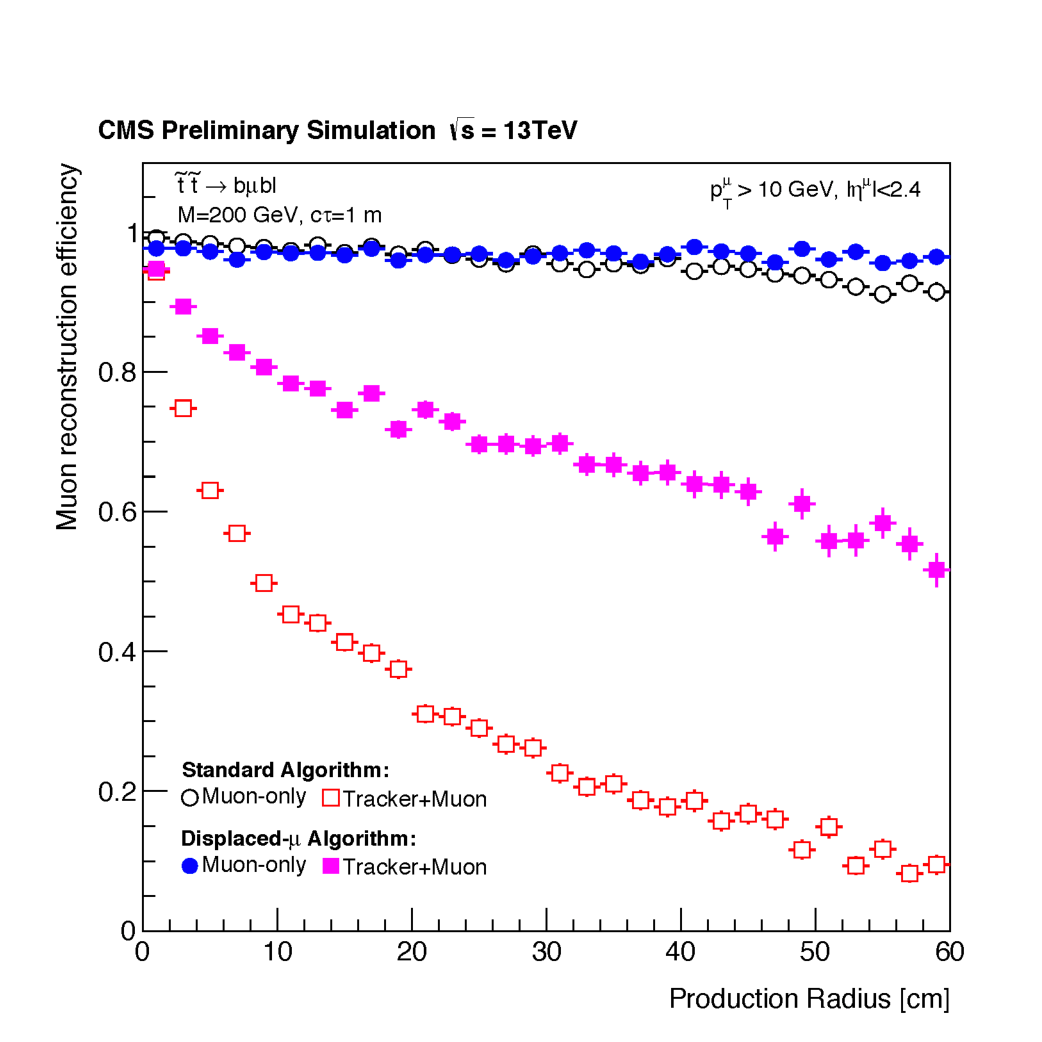
\includegraphics[clip,trim=0cm 0cm 0cm 2cm, width=0.48\textwidth]{Figures/c2/newreco.pdf}
  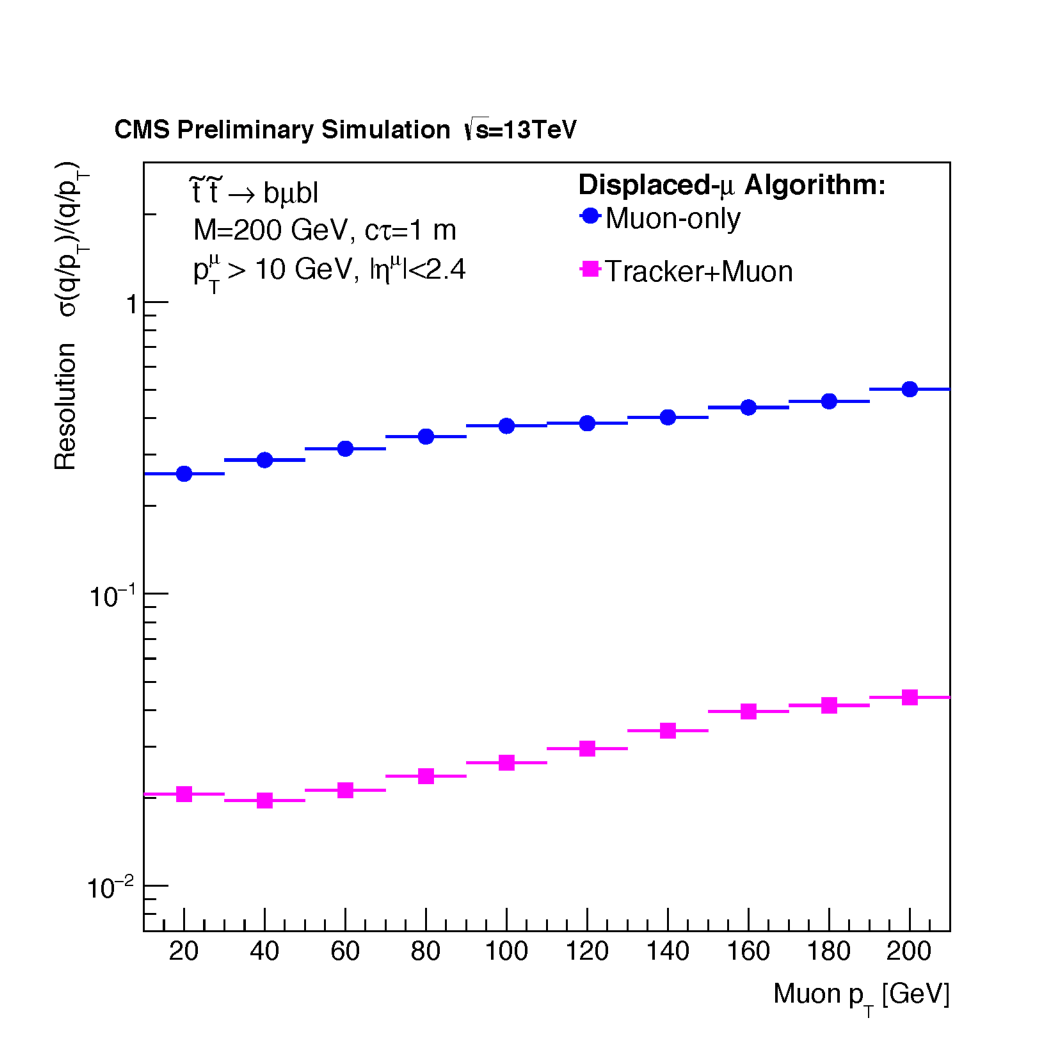
\includegraphics[clip,trim=0cm 0cm 0cm 2cm, width=0.48\textwidth]{Figures/c2/newreco2.pdf}
  \caption{Left, standard algorithms for muon-only (black) and tracker+muon (red) reconstruction,
compared with the new algorithms for displaced-muon reconstruction: Displaced
Standalone (blue) and Displaced Global
(magenta). Right, the resolution for the Displaced Standalone algorithm (blue) is shown in comparison
with that of the Displaced Global algorithm (magenta)~\cite{CMS-DP-2015-015}.}
  \label{fig:newreco}
\end{figure}

Figure~\ref{fig:newreco} (left) showns the muon reconstruction
efficiency for the two new algorithms in comparison with respect to
the standard ones. The comparison is done in 
simulated samples~\footnote{Simulated signal process: PYTHIA8 stop 
  pair ($\tilde{t}\tilde{t}$) production, $M(\tilde{t}) = 200$\GeV and
$c\tau=1$m. Decay $\tilde{t} \rightarrow b + \ell$} with displaced and
delayed~\footnote{Out-of-time or delayed muons indicate muons with significant delay with respect to the time of the
interaction.} muons, measuring the efficiency as function of the production radius, for muons from
the direct decay $\tilde{t} \rightarrow b + \ell$. A noticeable
improvement can be appreciated in the efficiency for displaced muons
using the new algorithms. In Figure~\ref{fig:newreco} (right) it is
measured the transverse momentum resolution ($\nicefrac{q}{\pt}$) as
function of the muon \pt for displaced muons from the direct decay $\tilde{t} \rightarrow b + \ell$.\\
The performance plots shown in Figure~\ref{fig:newreco} present bright
perspectives for the future of long-lived analysis involving
displaced muons. 

\subsection{Electron reconstruction}\label{sec:c2ele}

\subsubsection{Electron track reconstruction}\label{sec:trackele}

Electron PF objects are reconstructed with the PF algorithm 
based on the combination of tracker tracks and energy clusters in the 
ECAL, taking into consideration the sizeable fraction
of electron energy which is emitted in the form of bremsstrahlung photons while
crossing the tracker material~\cite{CMS:particleflow}. The bremsstrahlung radiation is collected
by organizing
\begin{wrapfigure}{r}{0.5\textwidth}
\centering
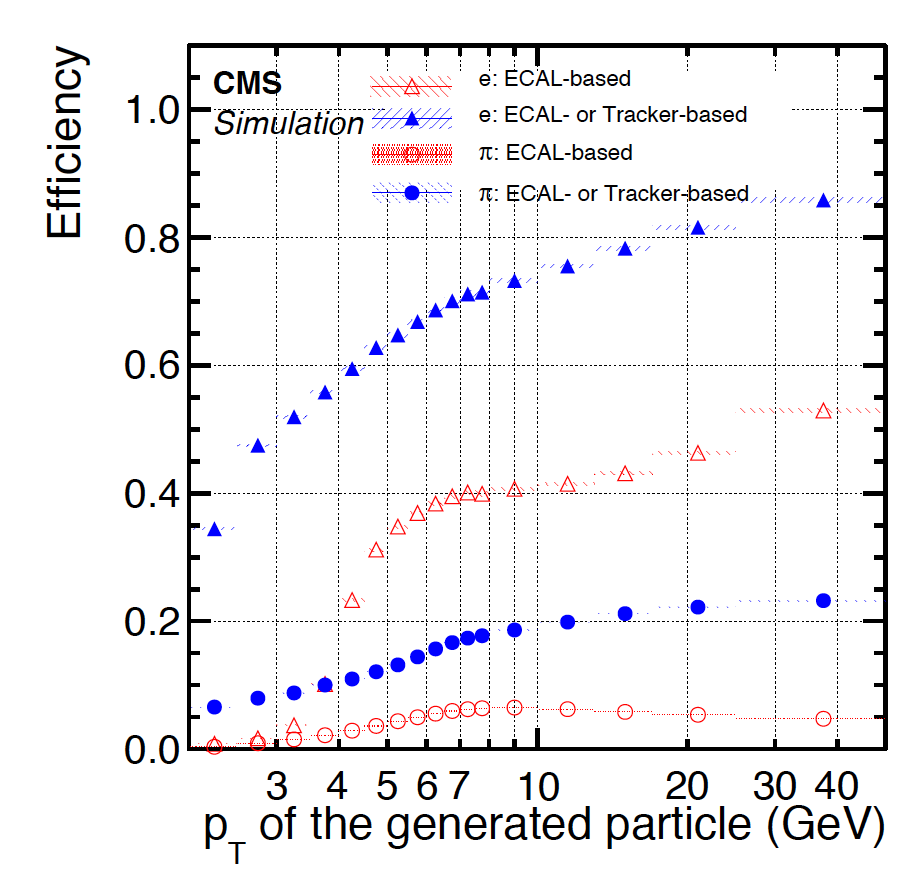
\includegraphics[width=.48\textwidth]{Figures/c2/eleecal}
  \caption{The electron seeding efficiency for electrons (triangles) and pions (circles) as a
function of \pt are shown. Both the efficiencies for ECAL-based
seeding only (hollow symbols) and with the tracker-based seeding added
(solid symbols) are shown~\cite{CMS:particleflow}.}
  \label{fig:c2ele}
\end{wrapfigure} 
 into a supercluster the ECAL clusters which are
reconstructed in a narrow window in $\eta$ and a wider window in $\phi$ along the electron direction (azimuthal
bending in the magnetic field).
For small \pt electrons, the ECAL supercluster approach can give
incorrect information regarding the total energy. The soft tracks are
significantly bent in the tracker by the magnetic field and the
radiated energy is dispersed over an extended area that the energy
deposits are not all
included in the supercluster. The missed deposits distort the correct
position of the supercluster and impede the proper match between
supercluster and corresponding hits in the innermost tracker layers.
Thus the \emph{tracker-based} electron seeding
method~\cite{CMS:particleflow} is introduced to complement and improve
the ECAL-based approach. Figure~\ref{fig:c2ele} shows the increase in efficiency caused by the tracker-based approach for electrons in b quark jets.\\
The final electron tracks are built using the Gaussian Sum Filter
(GSF) fitting (details in references~\cite{CMS:particleflow, Adam_2005}) which is more optimal to electrons than the Kalman-filter used
in the iterative tracking (refer to
Section~\ref{sec:trackvertex}). The GSF approach gives adequate
performances both for large (\ie soft electrons) and small (\ie high \pt electrons) amounts of radiated energy in the
tracker material.

The tracker-based seeding technique is effective at selecting $e^{-}$-$e^{+}$ coming from $\gamma$ conversions
in the tracker material, for both prompt and bremsstrahlung
photons. The possibility to correctly associate the converted
bremsstrahlung photons
to the their parent electrons is key in avoiding energy double
counting in the electron PF reconstruction~\cite{CMS:particleflow}. The proper identification
of the electrons from $\gamma$ conversions
in the tracker material becomes crucial for background description. In
the analyses presented in
Chapters~\ref{Chapter5} and~\ref{Chapter6}, the so-called
``conversion'' background has a major contribution and its correct
understanding is critical for good background
predictions.

Electrons are reconstructed within the geometrical acceptance of the
CMS tracking system, $|\eta|<2.5$.

\subsubsection{Electron identification}\label{sec:c2keleid}
In CMS detector there are different sources of electrons aside from the
prompt ones produced in the collision at the PV. Electrons can be
originated from either $\gamma$ conversions or from the decay of heavy-flavor
hadrons, additionally they can also be misidentified jets due to poor
reconstruction. It is necessary to implement a selection based on quality and
kinematic parameters,  in order to discriminate between different 
sources and to identify the
prompt electrons from the hard scattering.
Identification criteria are based on the shape of the electromagnetic shower
(which is usually smaller than hadronic shower), on the ratio between the
HCAL deposits and the ECAL ones and on a few track properties.\\
A method to distinguish between prompt and background
electrons is the adoption of a multivariate
analysis (MVA) classifier, trained in data and simulated events. In the MVA approach~\cite{mvatwiki}, a
single discriminator variable is built; it is computed based on
multiple variables of the electron object and it provides the best
separation between the signal and backgrounds. The output of the MVA
can be used to introduce a sharp cut to reject a portion of electrons
or it can be used, as distribution of the values, for a shape based
statistical analysis.\\
Another possibility is a simple set of criteria which have to be
all satisfied. This approach can be called \emph{cut-based}
identification (ID)~\cite{cutbasedtwiki}. The average efficiency for MVA
ID depends on the chosen discriminator working point, it can be 80\% or
90\%~\cite{mvatwiki}. For the cut-based ID there are few benchmark selection levels
which have efficiency equal to 90\% (\emph{loose ID}), 80\% (\emph{medium
  ID}) and 70\% (\emph{tight ID})~\cite{cutbasedtwiki}.

The efficiencies of the electron reconstruction and identification are
estimated in data and simulation events with a \emph{tag-and-probe}
method (refer to~\ref{sec:c2effmuon}).\\

As for muon case (refer to Section~\ref{sec:muoniso}), for electrons
the relative PF isolation can be evaluated as well. The electron
relative isolation is an essential discriminating variable against 
electrons originating from heavy-flavor hadron decays.


\subsubsection{Displaced electrons
  identification}\label{sec:c2dispele}
\begin{figure}[h]
\centering
  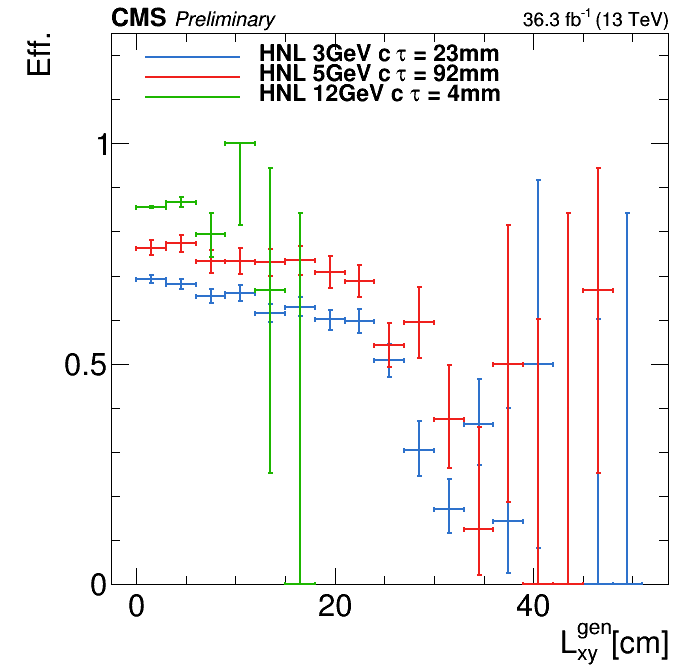
\includegraphics[width=0.45\textwidth]{Figures/c2/_e_l2id_Lxy_eff.png}
  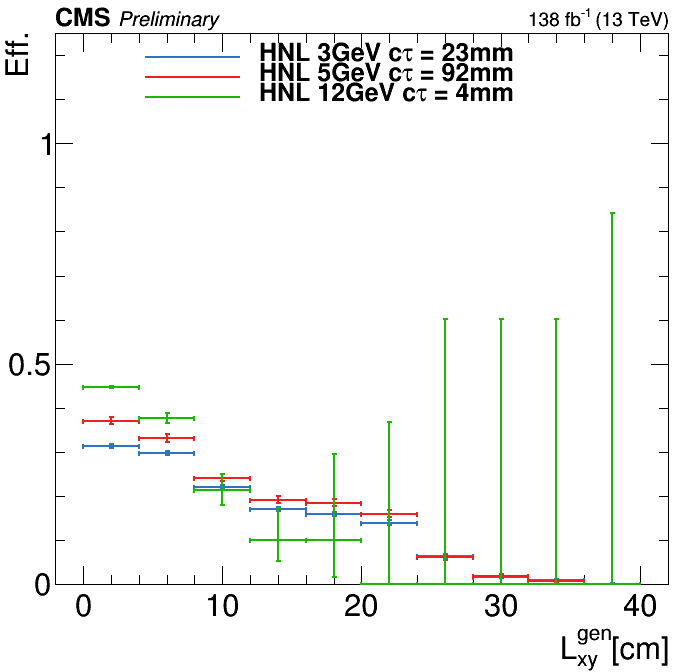
\includegraphics[width=0.45\textwidth]{Figures/c2/el_l2full_Lxy_eff.png}
  \caption{On the left, the pure ID efficiency with
    respect to GSF reconstructed tracks is shown. On the right the efficiency
    of reconstructed and identified electrons with
    respect to generated electrons is shown. \basile}
  \label{fig:basileele}
\end{figure}

The reconstruction of displaced electron objects is more challenging
with respect to the muon one. 
The main reason is the fact that for electron track reconstruction
there is not a corresponding algorithm to the muon standalone track
reconstruction. This latter allows a longer lever in the track
reconstruction procedure and it expects hits
further from the interaction point. The GSF tracks are then less
adaptable and optimal for displaced lepton scenarios.\\

The investigations presented in this paragraph are done in the context
of the long-loved heavy neutral lepton analysis presented in
Chapter~\ref{Chapter6}. They are circumscribed
to this specific scenario and they are not optimized for a more extended
implementation.  

\Displ electrons are identified using the \emph{cut-based loose ID}
but with fewer requirements. Two criteria have been removed because
they could affect the efficiency for electrons
not emerging from the primary vertex. \\
The conversion veto requirement which identifies
secondary vertices where $e^{-}$-$e^{+}$ pairs 
originate from $\gamma$ conversions in the tracker material is excluded.\\
Finally the request of the on the maximum number of
missing inner tracker hits it is removed in order to accommodate 
eventual larger displacements. \\
In Figure~\ref{fig:basileele}, on the left, the pure
identification efficiency with respect to the
reconstructed tracks is shown. It is estimated as function of the flight
distance, $L_{xy}$ of the long-lived particle. In the right figure
(~\ref{fig:basileele}), the ID efficiency is convoluted with the
reconstruction efficiency of the GSF tracks; hence the values are
computed with respect to the number of
generated tracks. For this specific case, three heavy neutral lepton
benchmark models are used with different neutrino masses (3, 5 and
12\GeV) and different lifetime values.

\clearpage
\section{Secondary vertex reconstruction} \label{sec:c2sv}

For the search for long-lived HNLs, presented in
Chapter~\ref{Chapter6} supplementary and
tailored treatment of the secondary vertex reconstruction and
identification is necessary. The SV is the decay vertex of the heavy
neutral lepton and it is the point of origin of its decay products.
\begin{wrapfigure}{r}{0.5\textwidth}
\centering
  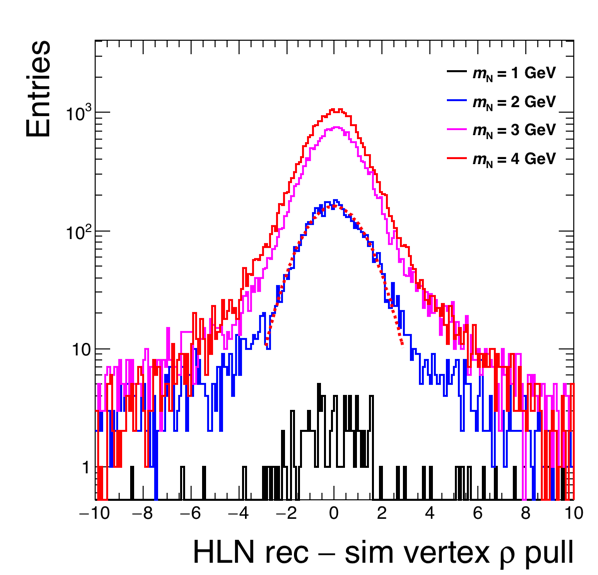
\includegraphics[clip,trim=1.cm 0cm .5cm 1.3cm, width=.38\textwidth]{Figures/c2/leptons_fromN_fromNW_vtx_rho_pull.png}
  \caption{Pull distributions of the
    transverse distance of the fitted SV from
    the PV, for HNL masses from 1 to 4\GeV,
    all with $\mixpar=10^{-4}$. The red curve overlaid to the blue
    histogram shows a Gaussian fit. \dani}
  \label{fig:svPulls}
\end{wrapfigure} 

In this specific case (~\ref{sec:llanalisi}), exactly two leptons, muon and/or electron, are
expected to originate from the SV. The SV reconstruction is done a
posteriori after the identification of the two lepton candidates which
are believed to be displaced. \\
The SV is found by fitting the two tracks to a common point with a Kalman-filter
approach~\cite{BILLOIR1990219}, using the \texttt{KalmanVertexFitter}
class implemented in the CMS reconstruction software (\texttt{CMSSW}).
The class returns the least-$\chi^2$ estimator of the two-track vertex
position and covariance matrix, along with the $\chi^2$ of the fit, as
an indicator of its goodness.
Figure~\ref{fig:svPulls} shows the pulls of the distance of the fitted
secondary vertex (SV) from the PV of the interaction projected on the
transverse plane (denoted as $\rho$). The pulls
are computed as the difference between the measured distance, $\rho$
and its true value from simulation, divided by the uncertainty
on the measured value. A standard deviation of about 1.2 is found from
a Gaussian fit to the pull distributions, revealing a slight
underestimation of the uncertainties.
\begin{figure}[h!]
  \centering
  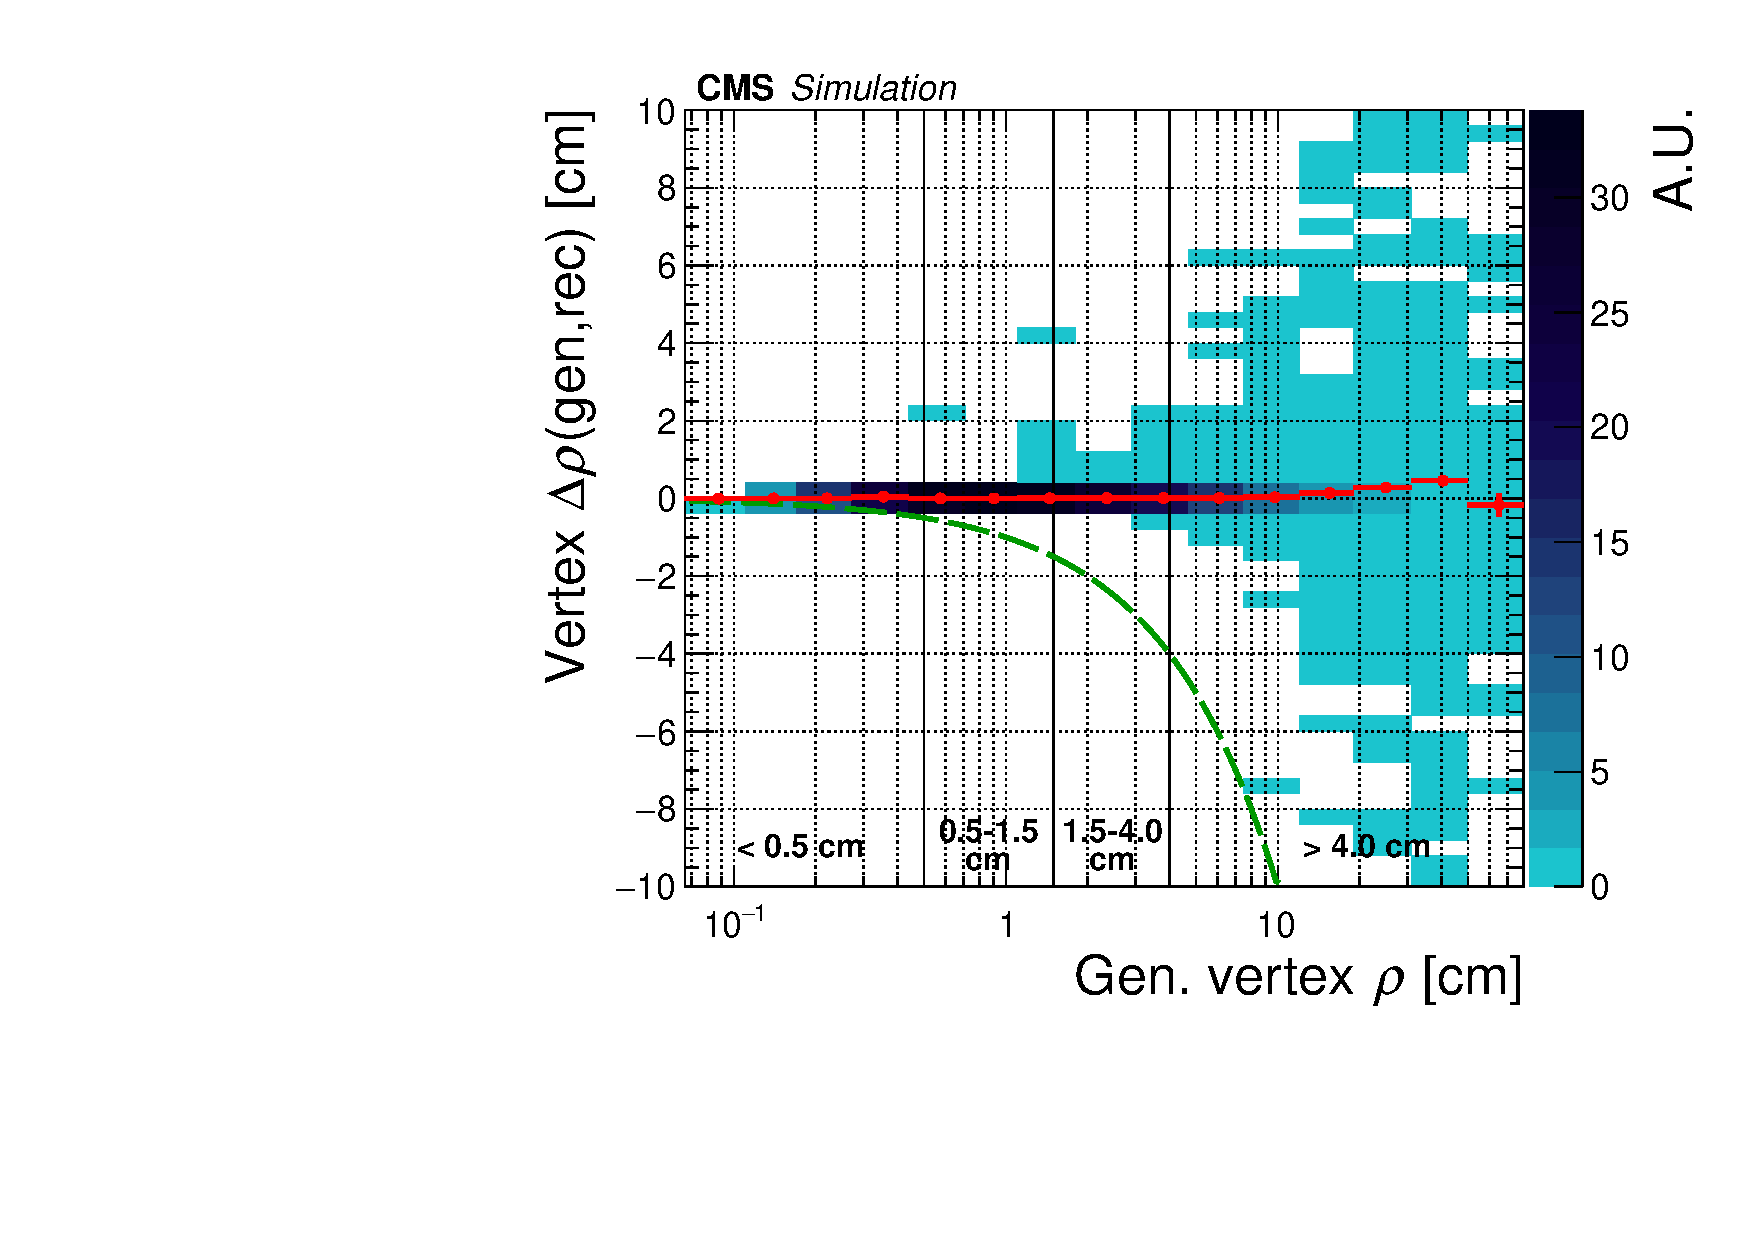
\includegraphics[width=.4\textwidth]{Figures/c6/selection/genvtx_recvtx_Drho_vs_rho_afterSel_zoom.pdf}
  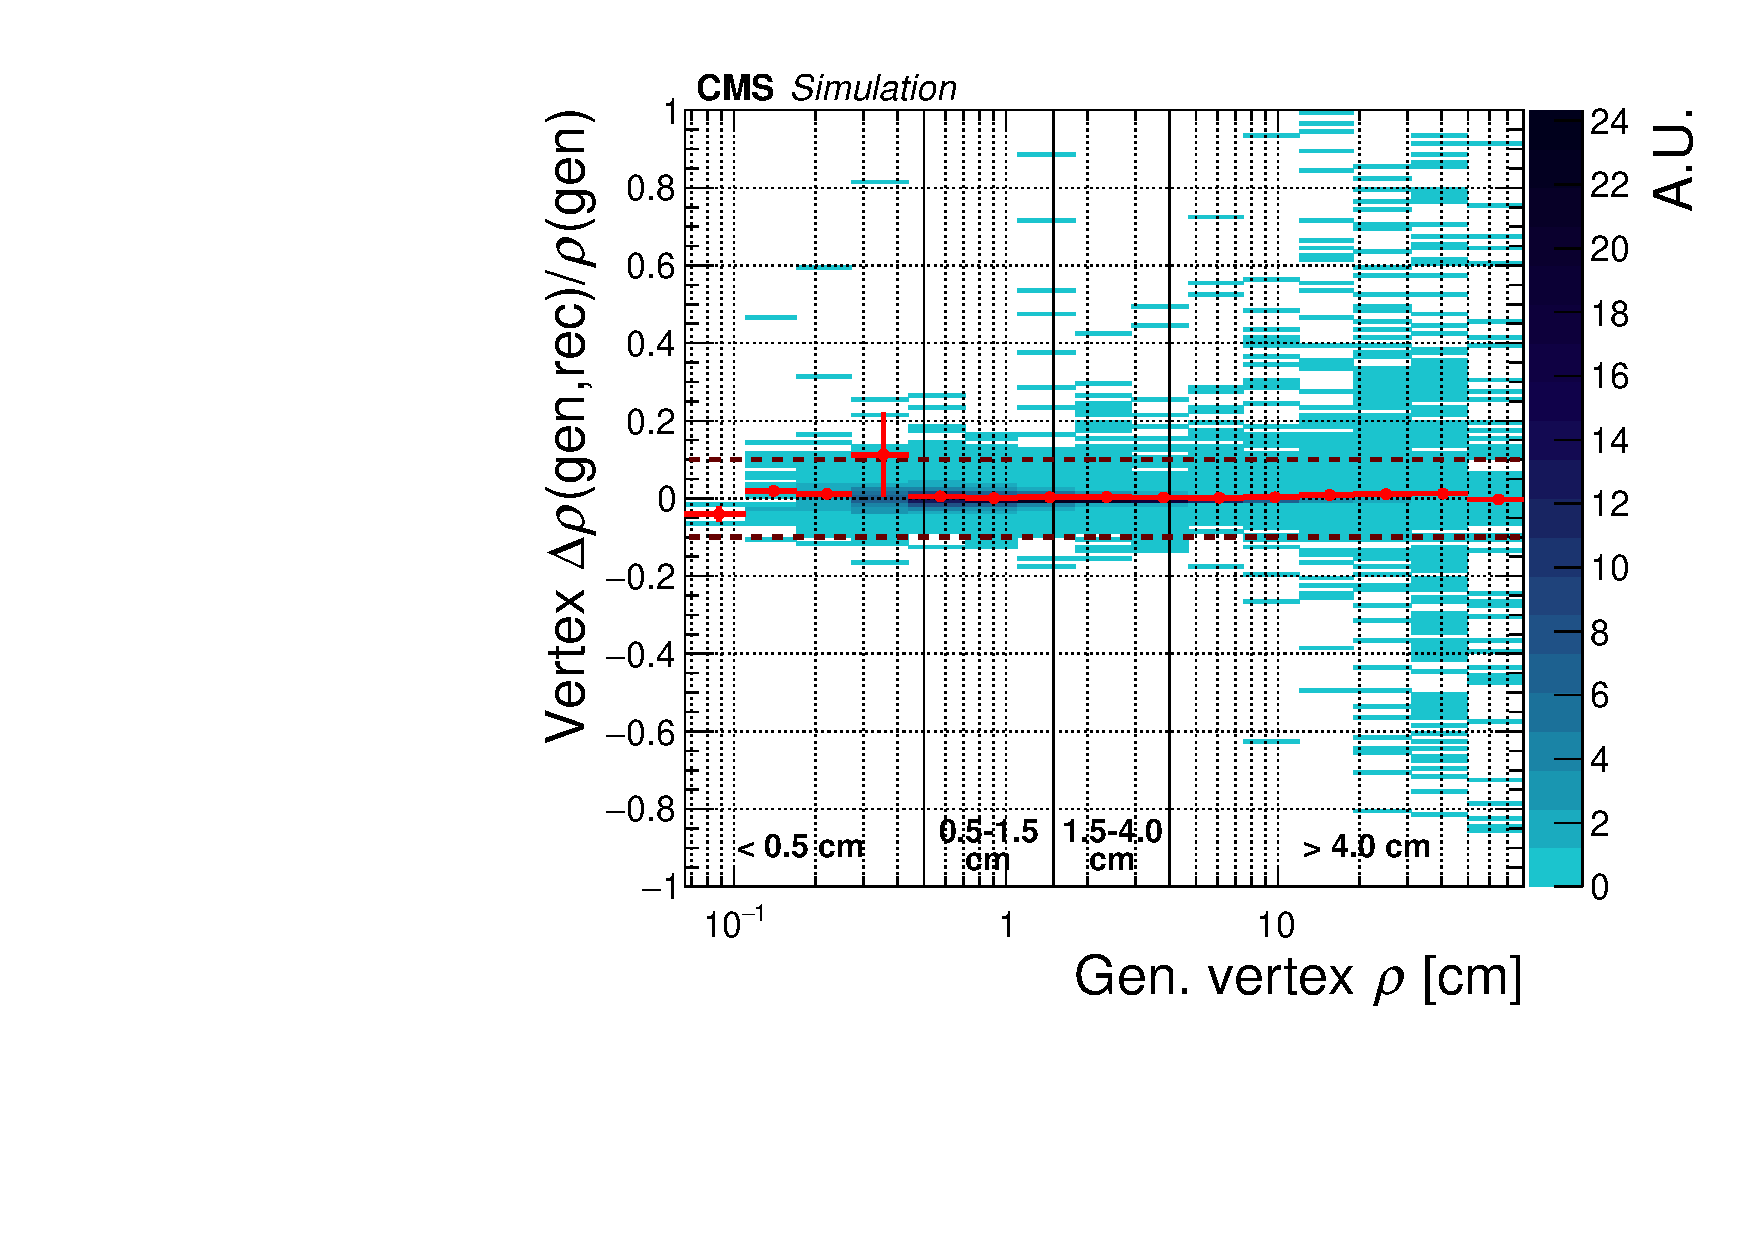
\includegraphics[width=.4\textwidth]{Figures/c6/selection/genvtx_recvtx_RelDrho_vs_rho_afterSel_zoom.pdf}
  \caption{Residuals (left) and relative residuals (right) of the
    transverse distance $\rho$ between the fitted secondary vertex and
    the PV of the interaction, as a function of the true $\rho$ value
    from simulation. 
    The red graph shows the mean value of the
    residuals in each $\rho$ bin and the uncertainty on the mean
    value. The dashed green line in the left plot indicates the
    distance between the generated primary and secondary vertices: any
    reconstructed vertex below this line would lie in the ``wrong''
    hemisphere, opposite to the direction of flight of the HNL.
    The horizontal dashed lines in the right plot delimit the region
    where $\Delta\rho(\mathrm{gen,rec})$ is less than 10\% of
    $\rho(\mathrm{gen})$. This region contains more than 99\% of
    the events for $\rho>0.5$cm, and about 97.4\% for $\rho<0.5$cm.
    \dani}
  \label{fig:svResidVsRho_all}
\end{figure}

To verify the accuracy of the reconstructed SV position, the residuals of the
transverse PV--SV distance $\rho$ with respect to the true generated
value, $\Delta\rho(\mathrm{gen,rec})$ and the relative residuals
$\Delta\rho(\mathrm{gen,rec})/\rho(\mathrm{gen})$ are studied as a
function of the true $\rho$. The results are shown in
Figure~\ref{fig:svResidVsRho_all}.

No significant biases are observed and
the tails are small: the fraction of events with
$\Delta\rho(\mathrm{gen,rec})/\rho(\mathrm{gen})$ larger than
10\%---indicated by the dashed horizontal lines in
Figure~\ref{fig:svResidVsRho_all} (right)---is about 2.6\% for $\rho<0.5\cm$, and less than 1\% for larger
displacements.

The quality of the reconstructed SVs is checked with specific
variables described in Section~\ref{sec:c2IP} such as the fit
probability and $\chi^2$ of the fit. 

The efficiency for this two-tracks-SV reconstruction is nearly 100\%.


\section{PF object and event identification
  variables}\label{sec:c2variables}
Aside from the variables introduced up to this point, there are additional
ones which are worth introducing at this stage of this dissertation. 
The list of variables presented in the next two sections is
contingent on the specification and parameters of the two data analyses presented in Chapters~\ref{Chapter5}
and~\ref{Chapter6}.\\
There are a number of variables which are referred specifically to light
leptons, electrons and muons, in particular those that are indicative
of the HNL flight distance.\\
A second set consists of a few event-based observables. 



\subsection*{Light lepton
  identification} \label{sec:c2leptonvariables}

\paragraph{Vertices and impact parameter variables.} \label{sec:c2IP}
Prompt leptons originate from the PV of the pp collision, hence they
are expected to have very modest impact parameters with respect to the
PV. On the contrary, nonprompt leptons and displaced leptons have
quite considerably large impact parameters due to the decay length of the
corresponding parent particles (partons or heavy neutral leptons).

\begin{figure}[h!]
\centering
  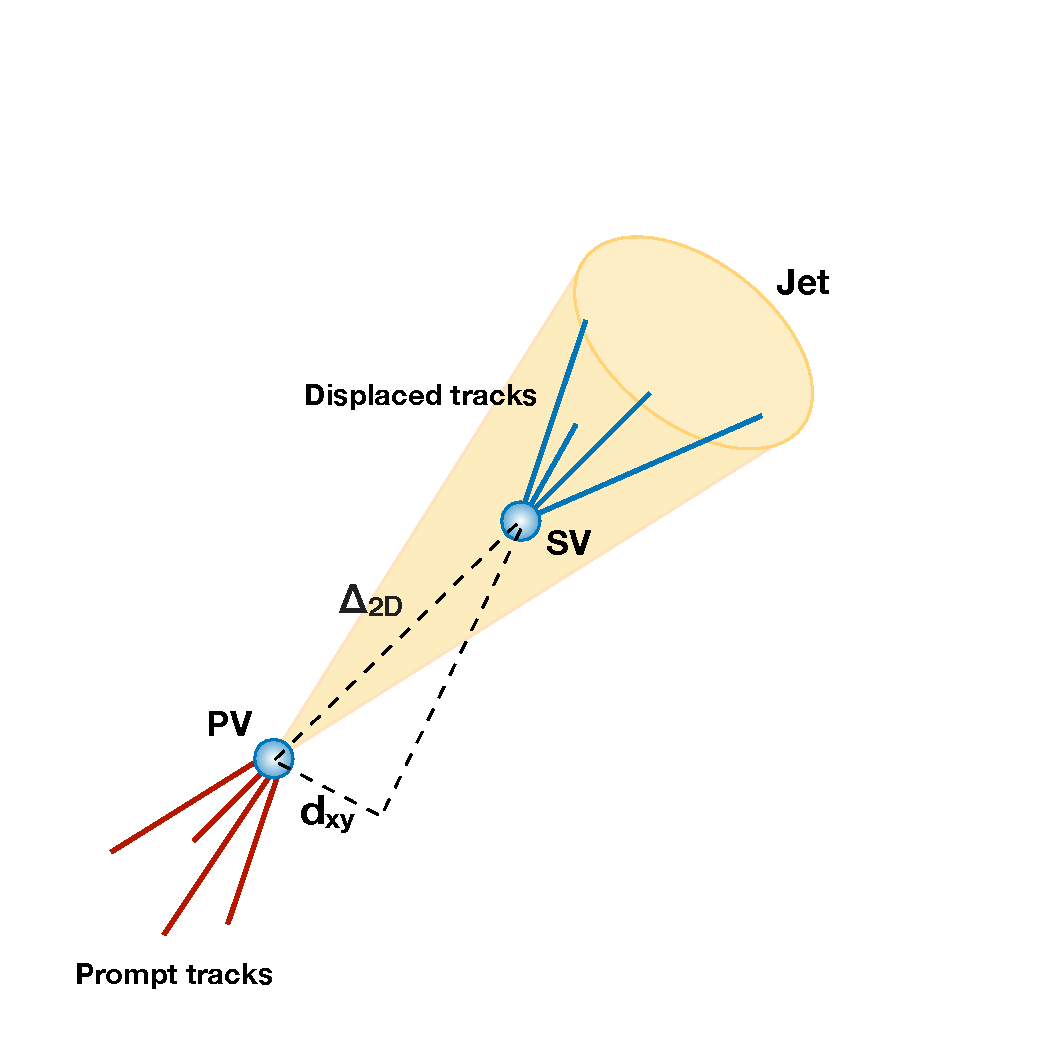
\includegraphics[clip,trim=1cm 0cm 3cm 4cm, width=0.58\textwidth]{Figures/c2/grafico.pdf}
  \caption{Schematic representation of the impact parameters variables.}
  \label{fig:impact}
\end{figure}

In the context of this thesis work, the following variables are used:
\begin{itemize}
%\setlength\itemsep{-0.1em}
\item $\boldsymbol{d_{xy}}$, impact parameter in the $x-y$ plane;
\item $\boldsymbol{d_z}$, impact parameter component in the the
  longitudinal direction, $z$-axis;
\item $\boldsymbol{SIP_{3D}}$, significance of the 3D impact parameter, $d_{3D}$
 . It is defined as the ratio between the $d_{3D}$ and its
  uncertainty; 
\item $\boldsymbol{\Delta_{2D}}$, the 2D distance between the PV and
  the SV. It is an optimal proxy to estimate the point of origin of the
displaced lepton and the heavy neutral lepton decay length. It is
computed as $\Deltwod = \sqrt{(x_{SV}-x_{PV})^{2} + (y_{SV}-y_{PV})^{2}}$;
\item $\boldsymbol{ S(\Delta_{2D})}$, the significance of the transverse distance
  between PV and SV, defined as the ratio of the transverse PV-SV
  distance $\Delta_{2D}$ and its uncertainty;
\item $\boldsymbol{ p_{SV}}$, SV probability. The quality of the reconstructed SV
  necessarily correlates with the precision on the track parameters of
  the two leptons in the SV, as well as the spatial separation between their
  trajectories at the intersection point. The SV quality is estimated as a probability based on the
$\chi^2$~fit from the kinematic vertex fitter;
\item $\boldsymbol{d}$, displacement. It is used to study the electron
  reconstruction performance where electrons originate from convert
  photon.
It is computed as: $d = \sqrt{2R d_{xy}+d_{xy}^2}$ where $R$ is the radius of curvature of
  the path of the nonprompt electron in magnetic field. This variable represents a suitable
  proxy to the actual displacement of the converted photon with
respect to the PV, and is also correlated with the $\Delta_{2D}$ variable.
\end{itemize}


\paragraph{Lepton isolation}\label{sec:c2iso}
To discriminate between prompt leptons and leptons coming from either the decays
of heavy-flavor hadrons or the decay in flight of charged $\pi^{\pm}$s and kaons, the isolation variable appears to be one of
the most critical variable to use. The PF isolation of a reconstructed
leptons is defined relative to its \pt as the scalar
sum of the energy of all the PF candidates emitted around the
direction of the lepton in the cones, $\Delta R = \sqrt{(\Delta
  \phi)^2+(\Delta \eta)^2}$, surrounding the object. It is computed as:
\begin{linenomath}
  \begin{equation}
    \label{eq:c2irel}
    \Irel = \frac{1}{\pt^\ell}
    \left(\sum_{ch.hadr.}\pt^{\mathrm{PV}} +
    \max{\left[0, \sum_{neu.hadr.}\pt + \sum_{pho.}\pt
        - \rho\cdot A_{\mathrm{eff}}\right]}\right)
  \end{equation}
\end{linenomath}
For the estimation of the PF isolation~\cite{CMS:particleflow}, it is computed the sum of the
\pt of charge hadrons and the \pt of neutral particles (hadrons
and photons) originating from the PV. Typical values used for  $\Delta
R$ are 0.3 and 0.4.\\
The term $\rho\cdot A_{\mathrm{eff}}$ is used to mitigate the
contribution of pileup to the isolation calculation: the average
transverse-momentum flow density $\rho$ is calculated in each event
using a ``jet area'' method~\cite{CACCIARI2008119}, and the effective
area $A_{\mathrm{eff}}$ is the geometric area of the isolation cone
times an $\eta$-dependent correction factor. This correction factor is applied to account for the contribution from pileup to the
neutral particles component~\cite{Sirunyan_2018_muon}.


\subsection*{General observables} \label{sec:c2observables}
\paragraph{Missing transverse momentum,
  $\boldsymbol{\ptmiss}$.}\label{sec:c2ptmiss}
Neutral leptons do not interact with any material of the CMS
sub-detectors, thus they leave the detector unseen. Nevertheless they
carry momentum energy which have to be estimated or else it would
create a sizable momentum imbalance in the transverse plane. The
transverse momentum of the initial state is zero. Hence, the sum of 
momenta of all objects in the transverse plane is
expected to be zero except for events where undetected particles are
created. From this missing balance is possible to estimate the energy
carried out by the neutrinos. \\
The \ptmiss is obtained as the magnitude of the negative vector sum of the transverse momenta of 
all reconstructed PF candidates and is further adjusted to account for
jet energy corrections applied to the event~\cite{CMS-PAS-JME-16-004}.
\begin{linenomath}
  \begin{equation}
    \label{eq:c2ptmiss}
    \overrightarrow{p}_T^{\text{miss}} \: = \: \sum \overrightarrow{p}_T,
    \;\;\; \;\;\; p_T^{\text{miss}} \: = \: |\overrightarrow{p}_T^{\text{miss}}|
  \end{equation}
\end{linenomath}

%%%%%%%%%%%%%%%%%%%%%%%%%%%%%%%%%%%%%%%%%%%%%%%%%%%%%
\clearpage
\section{Summary}\label{sec:summaryC3}

In this chapter the event reconstruction and lepton identification are discussed.\\
With a clear focus on light leptons, we described the reconstruction
of physics objects by using combined information from all the CMS
subsystems. In this context we
described in details of the PF algorithm with its input as output such as
leptons. \\
We addressed the identification and characterization aspects of the
reconstructed physics objects. We listed the main identification
variables and the related levels of tagging efficiencies.
According to the desired compromise between efficiency and purity, 
for electrons and muons a set of different variables and selections definitions
are defined.

In this chapter extensive attention is paid 
to detail the algorithms and strategies adopted to
correctly reconstruct and identify displaced vertices, muons and
electrons. \\
The CMS centralized displaced object algorithms are
described as well as the specific IDs and methods which were developed in
the context of this thesis. I have contributed to this latter part. The second year of my PhD was dedicated
exclusively to the study, understanding and identification of
displaced objects. In particular, I have contributed to the
decision of valuable variables and features to selected displaced muons with
high efficiency and low misidentification rates. The exotica long-lived working group was the
setting for these developments and several improvements were presented
and discussed there by myself. The comprehensive
insights acquired during the analysis process were crucial during the
paper review and helped to formulate the interpretation of the
long-lived heavy neutral lepton results.\\
The displaced object descriptions are going to be central to grasp the
scope and the challenges of the analysis presented in
Chapter~\ref{Chapter6}. \\

A list of PF objects and event identification variables are added at
the end of this Chapter~\ref{Chapter2_5}; each of the variable will be found later on
the text.